% Options for packages loaded elsewhere
\PassOptionsToPackage{unicode}{hyperref}
\PassOptionsToPackage{hyphens}{url}
%
\documentclass[
]{article}
\usepackage{amsmath,amssymb}
\usepackage{lmodern}
\usepackage{iftex}
\ifPDFTeX
  \usepackage[T1]{fontenc}
  \usepackage[utf8]{inputenc}
  \usepackage{textcomp} % provide euro and other symbols
\else % if luatex or xetex
  \usepackage{unicode-math}
  \defaultfontfeatures{Scale=MatchLowercase}
  \defaultfontfeatures[\rmfamily]{Ligatures=TeX,Scale=1}
\fi
% Use upquote if available, for straight quotes in verbatim environments
\IfFileExists{upquote.sty}{\usepackage{upquote}}{}
\IfFileExists{microtype.sty}{% use microtype if available
  \usepackage[]{microtype}
  \UseMicrotypeSet[protrusion]{basicmath} % disable protrusion for tt fonts
}{}
\makeatletter
\@ifundefined{KOMAClassName}{% if non-KOMA class
  \IfFileExists{parskip.sty}{%
    \usepackage{parskip}
  }{% else
    \setlength{\parindent}{0pt}
    \setlength{\parskip}{6pt plus 2pt minus 1pt}}
}{% if KOMA class
  \KOMAoptions{parskip=half}}
\makeatother
\usepackage{xcolor}
\IfFileExists{xurl.sty}{\usepackage{xurl}}{} % add URL line breaks if available
\IfFileExists{bookmark.sty}{\usepackage{bookmark}}{\usepackage{hyperref}}
\hypersetup{
  pdftitle={Data Analysis Coursebook},
  pdfauthor={Marcell Granat \& Zoltan Madari},
  hidelinks,
  pdfcreator={LaTeX via pandoc}}
\urlstyle{same} % disable monospaced font for URLs
\usepackage[margin=1in]{geometry}
\usepackage{color}
\usepackage{fancyvrb}
\newcommand{\VerbBar}{|}
\newcommand{\VERB}{\Verb[commandchars=\\\{\}]}
\DefineVerbatimEnvironment{Highlighting}{Verbatim}{commandchars=\\\{\}}
% Add ',fontsize=\small' for more characters per line
\usepackage{framed}
\definecolor{shadecolor}{RGB}{248,248,248}
\newenvironment{Shaded}{\begin{snugshade}}{\end{snugshade}}
\newcommand{\AlertTok}[1]{\textcolor[rgb]{0.94,0.16,0.16}{#1}}
\newcommand{\AnnotationTok}[1]{\textcolor[rgb]{0.56,0.35,0.01}{\textbf{\textit{#1}}}}
\newcommand{\AttributeTok}[1]{\textcolor[rgb]{0.77,0.63,0.00}{#1}}
\newcommand{\BaseNTok}[1]{\textcolor[rgb]{0.00,0.00,0.81}{#1}}
\newcommand{\BuiltInTok}[1]{#1}
\newcommand{\CharTok}[1]{\textcolor[rgb]{0.31,0.60,0.02}{#1}}
\newcommand{\CommentTok}[1]{\textcolor[rgb]{0.56,0.35,0.01}{\textit{#1}}}
\newcommand{\CommentVarTok}[1]{\textcolor[rgb]{0.56,0.35,0.01}{\textbf{\textit{#1}}}}
\newcommand{\ConstantTok}[1]{\textcolor[rgb]{0.00,0.00,0.00}{#1}}
\newcommand{\ControlFlowTok}[1]{\textcolor[rgb]{0.13,0.29,0.53}{\textbf{#1}}}
\newcommand{\DataTypeTok}[1]{\textcolor[rgb]{0.13,0.29,0.53}{#1}}
\newcommand{\DecValTok}[1]{\textcolor[rgb]{0.00,0.00,0.81}{#1}}
\newcommand{\DocumentationTok}[1]{\textcolor[rgb]{0.56,0.35,0.01}{\textbf{\textit{#1}}}}
\newcommand{\ErrorTok}[1]{\textcolor[rgb]{0.64,0.00,0.00}{\textbf{#1}}}
\newcommand{\ExtensionTok}[1]{#1}
\newcommand{\FloatTok}[1]{\textcolor[rgb]{0.00,0.00,0.81}{#1}}
\newcommand{\FunctionTok}[1]{\textcolor[rgb]{0.00,0.00,0.00}{#1}}
\newcommand{\ImportTok}[1]{#1}
\newcommand{\InformationTok}[1]{\textcolor[rgb]{0.56,0.35,0.01}{\textbf{\textit{#1}}}}
\newcommand{\KeywordTok}[1]{\textcolor[rgb]{0.13,0.29,0.53}{\textbf{#1}}}
\newcommand{\NormalTok}[1]{#1}
\newcommand{\OperatorTok}[1]{\textcolor[rgb]{0.81,0.36,0.00}{\textbf{#1}}}
\newcommand{\OtherTok}[1]{\textcolor[rgb]{0.56,0.35,0.01}{#1}}
\newcommand{\PreprocessorTok}[1]{\textcolor[rgb]{0.56,0.35,0.01}{\textit{#1}}}
\newcommand{\RegionMarkerTok}[1]{#1}
\newcommand{\SpecialCharTok}[1]{\textcolor[rgb]{0.00,0.00,0.00}{#1}}
\newcommand{\SpecialStringTok}[1]{\textcolor[rgb]{0.31,0.60,0.02}{#1}}
\newcommand{\StringTok}[1]{\textcolor[rgb]{0.31,0.60,0.02}{#1}}
\newcommand{\VariableTok}[1]{\textcolor[rgb]{0.00,0.00,0.00}{#1}}
\newcommand{\VerbatimStringTok}[1]{\textcolor[rgb]{0.31,0.60,0.02}{#1}}
\newcommand{\WarningTok}[1]{\textcolor[rgb]{0.56,0.35,0.01}{\textbf{\textit{#1}}}}
\usepackage{longtable,booktabs,array}
\usepackage{calc} % for calculating minipage widths
% Correct order of tables after \paragraph or \subparagraph
\usepackage{etoolbox}
\makeatletter
\patchcmd\longtable{\par}{\if@noskipsec\mbox{}\fi\par}{}{}
\makeatother
% Allow footnotes in longtable head/foot
\IfFileExists{footnotehyper.sty}{\usepackage{footnotehyper}}{\usepackage{footnote}}
\makesavenoteenv{longtable}
\usepackage{graphicx}
\makeatletter
\def\maxwidth{\ifdim\Gin@nat@width>\linewidth\linewidth\else\Gin@nat@width\fi}
\def\maxheight{\ifdim\Gin@nat@height>\textheight\textheight\else\Gin@nat@height\fi}
\makeatother
% Scale images if necessary, so that they will not overflow the page
% margins by default, and it is still possible to overwrite the defaults
% using explicit options in \includegraphics[width, height, ...]{}
\setkeys{Gin}{width=\maxwidth,height=\maxheight,keepaspectratio}
% Set default figure placement to htbp
\makeatletter
\def\fps@figure{htbp}
\makeatother
\setlength{\emergencystretch}{3em} % prevent overfull lines
\providecommand{\tightlist}{%
  \setlength{\itemsep}{0pt}\setlength{\parskip}{0pt}}
\setcounter{secnumdepth}{5}
\usepackage{pdfpages}

\usepackage{booktabs}
\usepackage{amsthm}
\makeatletter
\def\thm@space@setup{%
  \thm@preskip=8pt plus 2pt minus 4pt
  \thm@postskip=\thm@preskip
}
\makeatother


% sidebar environment
\usepackage{framed,color}
\definecolor{shadecolor}{RGB}{242,242,242}
\makeatletter
\newenvironment{sidebar}{%
\medskip{}
\setlength{\fboxsep}{.8em}
 \def\at@end@of@kframe{}%
 \ifinner\ifhmode%
  \def\at@end@of@kframe{\end{minipage}}%
  \begin{minipage}{\columnwidth}%
 \fi\fi%
 \def\FrameCommand##1{\hskip\@totalleftmargin \hskip-\fboxsep
 \colorbox{shadecolor}{##1}\hskip-\fboxsep
     % There is no \\@totalrightmargin, so:
     \hskip-\linewidth \hskip-\@totalleftmargin \hskip\columnwidth}%
 \MakeFramed {\advance\hsize-\width
   \@totalleftmargin\z@ \linewidth\hsize
   \@setminipage}}%
 {\par\unskip\endMakeFramed%
 \at@end@of@kframe}
\makeatother
\ifLuaTeX
  \usepackage{selnolig}  % disable illegal ligatures
\fi
\usepackage[]{natbib}
\bibliographystyle{plainnat}

\title{\textbf{Data Analysis} Coursebook}
\author{Marcell Granat \& Zoltan Madari}
\date{}

\begin{document}
\maketitle

{
\setcounter{tocdepth}{2}
\tableofcontents
}
\pagebreak

\hypertarget{welcome}{%
\section*{Welcome}\label{welcome}}
\addcontentsline{toc}{section}{Welcome}

\emph{I hope this message finds you well.}

This is an online bookdown file, which we plan to \emph{update regularly} with the class material. We suggest that you to write the code simultaneously with us at seminar, but bugs can always occur out of the blue\ldots{} If you missed something or just want to revisit the topic with additional comments (probably before the exam day) this page is here to help.

At the end of the course you should know:

\begin{itemize}
\item
  What are data types, data quality, and data preprocessing?
\item
  What are the components of \texttt{tidyverse} and what are their advantage?
\item
  What are density, distribution function, quantile functions?
\item
  What are data clustering techniques?
\item
  What are the main techniques for association analysis?
\end{itemize}

We will work with \texttt{R}, one the most loved statistical programming language. Do not be afraid if you do not have any programming experience, this is a beginner course. However, by the end of the program, we hope you will find useful the concept and practical tips we offer, and you will be able to solve your own real life data analysis issues.

\hypertarget{syllabus}{%
\section*{Syllabus}\label{syllabus}}
\addcontentsline{toc}{section}{Syllabus}

\hypertarget{topics}{%
\subsection{Topics}\label{topics}}

\begin{itemize}
\item
  \textbf{Basic R knowledge (Week 1)}

  \begin{itemize}
  \item
    Data categorize, sampling, importing-exporting
  \item
    Types, tables, selection, objects, functions
  \end{itemize}
\item
  \textbf{Data manipulation in Tidyverse (Week 2)}

  \begin{itemize}
  \item
    Filter, group\_by, arrange, summarize commands
  \item
    \texttt{\%\textgreater{}\%}
  \item
    Join (mutating, filtering)
  \item
    tidy data (longer, wider)
  \end{itemize}
\item
  \textbf{Visualization with ggplot2 (Week 3)}

  \begin{itemize}
  \item
    Layers, facets, geoms
  \item
    Descriptive statistics in R
  \item
    Summary statistics, variability, correlation, covariance
  \item
    Extreme values, problem of missing values
  \end{itemize}
\item
  \textbf{Statistical estimation (Week 4)}

  \begin{itemize}
  \tightlist
  \item
    Distributions
  \item
    Sample techniques, confidence intervals, standard error
  \end{itemize}
\item
  \textbf{Hypothesis testing I (Week 5)}

  \begin{itemize}
  \item
    Inductive statistics in R
  \item
    Null and alternative hypothesis, t-test, p-value, fals
    positive/negative, Type I and II error
  \end{itemize}
\item
  \textbf{Hypothesis testing II (Week 6)}

  \begin{itemize}
  \tightlist
  \item
    Relation testing in R
  \end{itemize}
\item
  \textbf{Project presentations (Week 7)}
\end{itemize}

\hypertarget{requirements}{%
\subsection{\texorpdfstring{\textbf{Requirements}}{Requirements}}\label{requirements}}

\begin{itemize}
\item
  \textbf{Test} (30\%): 90 min task solution in R + explanation (exam week)
\item
  \textbf{Project} (25\%): groups (3-4 students), one detailed report
  (essay) and one - \textbf{presentation}
\item
  \textbf{Homeworks} and essays (45\%)
\item
  \textbf{Extra} tasks (+5\%)
\end{itemize}

\hypertarget{project}{%
\subsubsection{Project}\label{project}}

By the end of the course you have to make a statistical report about your own research project in small groups. You have to find a proper dataset (kaggle, eurostat, UCI datasets etc.) or conduct an own survey in optional topic.

At week 7 you will hold a presentation about your findings and results. At the end of the week you will upload your detailed essay about your project work.

\hypertarget{homework}{%
\subsubsection{Homework}\label{homework}}

During the Study period you get 3-5 homeworks. The number of homeworks depends ont he material progress. It could be R code writing or R code writing and analysis (short essay about methods and results).

\begin{longtable}[]{@{}ll@{}}
\caption{Grades}\tabularnewline
\toprule
\endhead
0-50\% & Fail (1) \\
51-62\% & Pass (2) \\
63-74\% & Satisfactory (3) \\
75-86\% & Good (4) \\
87-100\% & excellent (5) \\
\bottomrule
\end{longtable}

\hypertarget{recommended-compulsory-reading}{%
\subsection{Recommended (compulsory) reading}\label{recommended-compulsory-reading}}

\begin{itemize}
\item
  \href{http://r4ds.had.co.nz/}{\textbf{Grolemund G \& Wickham H:
  R for Data Science}}
\item
  Gábor Békés \& Gábor Kézdi: Data Analysis:
  Patterns, Prediction and Causality
\end{itemize}

\hypertarget{part-week-1}{%
\part*{Week 1}\label{part-week-1}}
\addcontentsline{toc}{part}{Week 1}

\hypertarget{lecture1}{%
\section{Lecture 1}\label{lecture1}}

\hypertarget{seminar1}{%
\section{Introduction to R}\label{seminar1}}

\hypertarget{why-r}{%
\subsection{Why R?}\label{why-r}}

In this chapter we will discuss the basics of R programming.
R is a free software, used by millions in the field of statistics, data science, economics and many others.

The R programming language is an important tool for data related tasks, but it is much more.
Just like other programming languages, R has many additional packages, which can extend its basic functionality.
R has a great (probably the best) graphical tools to create your charts, and with shiny, you can easily build your minimalist web applications.
We will learn about data manipulation, analysis and how to create awesome reports, like dashboards.

\hypertarget{layout}{%
\subsection{Setup}\label{layout}}

You can download R and RStudio from the official site of \href{https://www.rstudio.com/products/rstudio/download/\#download}{RStudio}.
Please install the appropriate version based on your OS, and do not forget that you also have to install R as well.

\href{https://www.rstudio.com/products/rstudio/download/\#download}{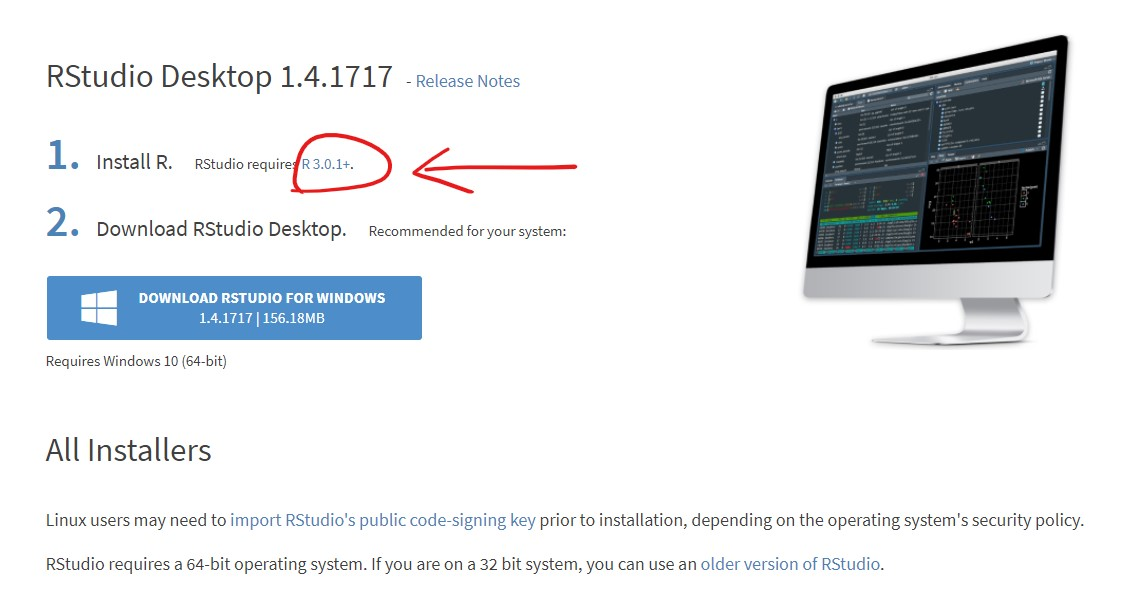
\includegraphics[width=6.25in,height=\textheight]{images/installr.jpg}}

\href{https://cran.rstudio.com/}{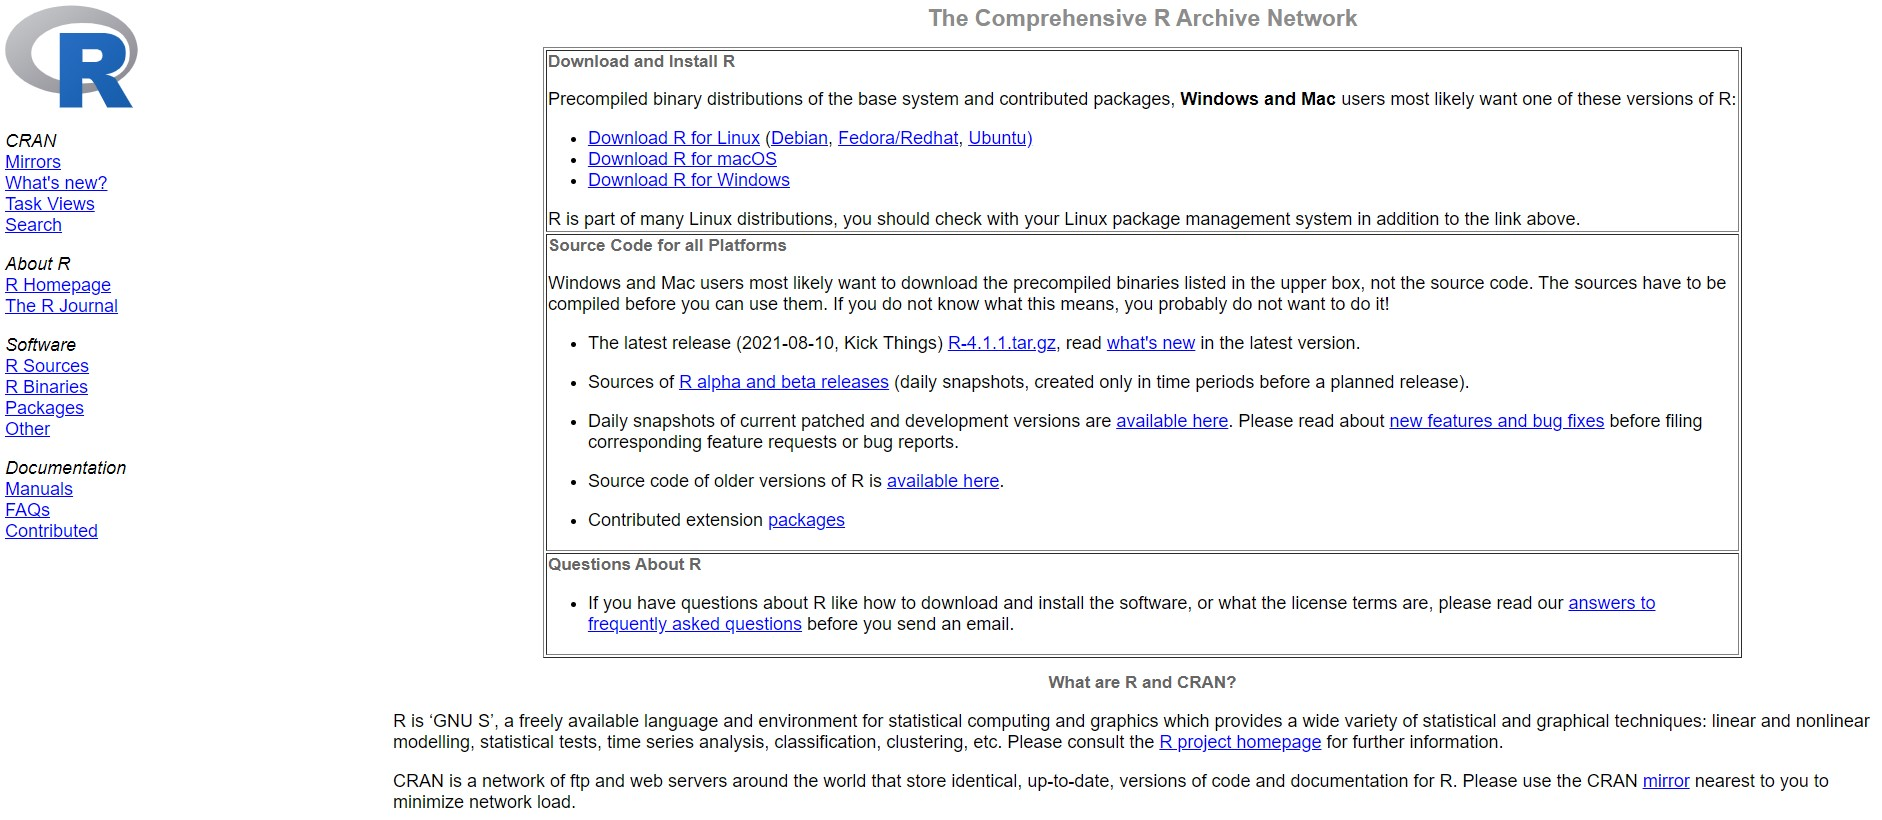
\includegraphics[width=6.25in,height=\textheight]{images/installr2.jpg}}

Run R's installer file after the downloading process is finished.
Next, we will also need the RStudio.

\href{https://www.rstudio.com/products/rstudio/download/\#download}{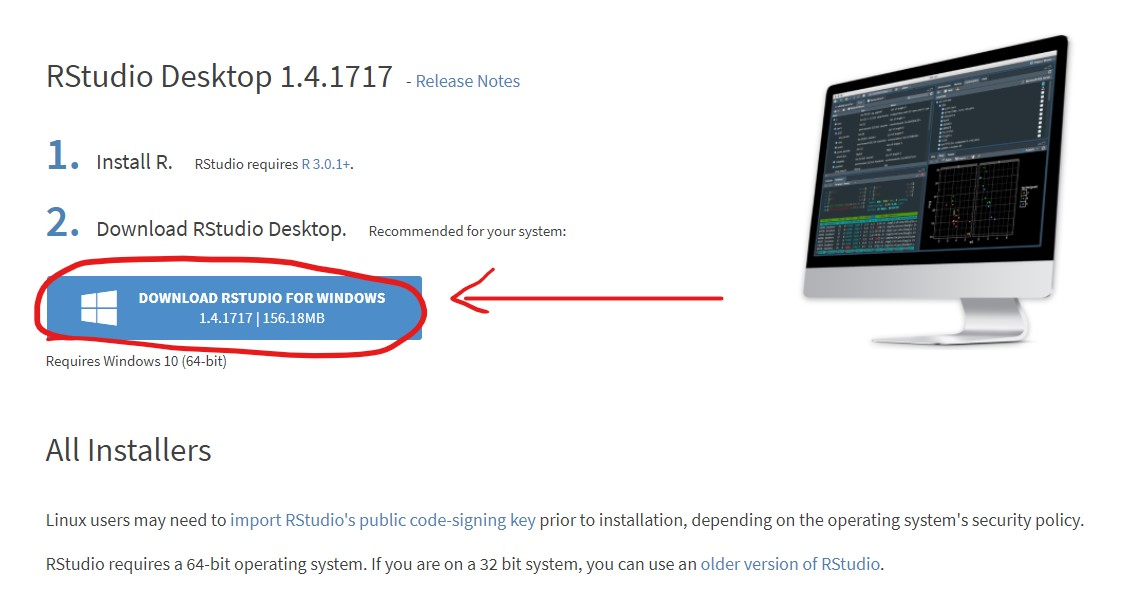
\includegraphics[width=6.25in,height=\textheight]{images/installr3.jpg}}

If the installation process of R and RStudio is finished, then we can open RStudio and start to learn the software.

\hypertarget{our-first-meet-with-r}{%
\subsection{Our first meet with R}\label{our-first-meet-with-r}}

RStudio is dedicated IDEE for R, which means, that it will make our life much simplier.
In stead of writing each line of code ourself, RStudio has many built-in functions to help us.
We see some panes if we open RStudio:

\begin{figure}

{\centering 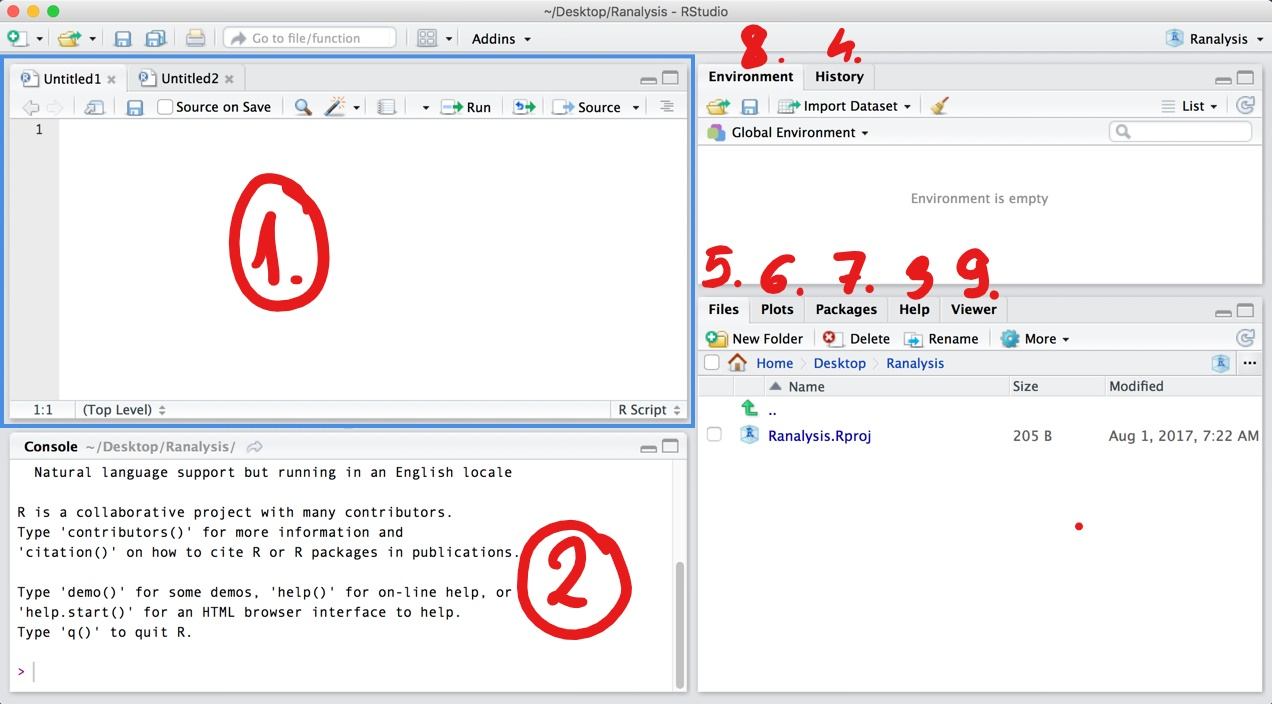
\includegraphics[width=0.7\linewidth]{C:/rprojects/Data-Analysis/images/Inkedrstudio_LI} 

}

\caption{Panes in RStudio}\label{fig:unnamed-chunk-3}
\end{figure}

\begin{enumerate}
\def\labelenumi{\arabic{enumi}.}
\item
  Source

  \begin{itemize}
  \tightlist
  \item
    We will write here our codes, which we would like to save.
    The basic extension of our codes are \texttt{.R}, but this is not the only possibility (we will cover this later). Once you save your code for later use, you can open your script also with a simple text editor (like Notepad), since this is only plain text. If you hit \texttt{enter} your code wont be executed, you will just simply start a new line. If you want to run your code hit \texttt{ctrl\ +\ enter} to execute a single line, and \texttt{ctrl+shift+enter} to execute your full script.
  \end{itemize}
\item
  Console

  \begin{itemize}
  \tightlist
  \item
    Here you find the executed codes, and the response to that. For example, if you type \texttt{2\ +\ 2} and hit \texttt{enter}, R will execute the expression, and response that it is 4.
  \end{itemize}
\end{enumerate}

\begin{Shaded}
\begin{Highlighting}[]
\DecValTok{2} \SpecialCharTok{+} \DecValTok{2}
\CommentTok{\#\textgreater{} [1] 4}
\end{Highlighting}
\end{Shaded}

\begin{enumerate}
\def\labelenumi{\arabic{enumi}.}
\setcounter{enumi}{2}
\item
  Help

  \begin{itemize}
  \tightlist
  \item
    You can use this pane if you are not familier with a function. For example, you want to know what input you can specify while using \texttt{mean}, you can type \texttt{?mean} on the console, or use the search field on this pane. The description of the function will be presented on this pane. (This pane is super useful on the exam)
  \end{itemize}
\item
  History
\item
  Files

  \begin{itemize}
  \tightlist
  \item
    You can see the list of your files which are in the current working directory. Working directory is the folder, from where R want currently read the files. If you want to import a dataset, just click on a file on this pane.
  \item
    I highly recommend you to set a project folder for the class and any later job. This means that, R creates a folder and puts an \texttt{.Rproj} file into it. You can always click on this \texttt{.Rproj} file to return your unfinished work. You can customise if R should put the variables into your environtent as you left them last time, you have a history about the used codes, and you see all the data you copy + paste into this folder.
  \end{itemize}
\item
  Plots
\item
  Packages

  \begin{itemize}
  \tightlist
  \item
    You can install packages from this pane. If you need a given package, click on install, and start typing its name. After that, you have to activate packages each time you open R again with the \texttt{library(eurostat)} command. You can also use a function from a package if you just simly type \texttt{eurostat::get\_eurostat()}.
  \end{itemize}
\item
  Environment

  \begin{itemize}
  \tightlist
  \item
    Here you can see the list of the variables you have already created. For example you can type \texttt{x\ =\ 3} on the console. Now and x variable will appear in the environment pane, and you can check its value if you type \texttt{x} on the console. You can also save these variables into an \texttt{.RData} data format if you wish.
  \end{itemize}
\item
  Viewer
\end{enumerate}

\hypertarget{data-types}{%
\subsection{Data types}\label{data-types}}

Lets see first, what kind of datatypes exist in R. Lets assign a variable called \texttt{x}.

\begin{Shaded}
\begin{Highlighting}[]
\NormalTok{x }\OtherTok{\textless{}{-}} \DecValTok{4}
\end{Highlighting}
\end{Shaded}

So, what is the type of \texttt{x}? We can use the \texttt{class} command to answer this.

\begin{Shaded}
\begin{Highlighting}[]
\FunctionTok{class}\NormalTok{(x)}
\CommentTok{\#\textgreater{} [1] "numeric"}
\end{Highlighting}
\end{Shaded}

Its numeric\footnote{Integer and double also exist in R, but these are not the default, and variables will be always coerced automatically}. This means that you can use \texttt{+}, \texttt{-}, \texttt{*} operators on it.

Lets see other types.

\begin{Shaded}
\begin{Highlighting}[]
\NormalTok{y }\OtherTok{\textless{}{-}} \StringTok{"blue"}
\FunctionTok{class}\NormalTok{(y)}
\CommentTok{\#\textgreater{} [1] "character"}
\end{Highlighting}
\end{Shaded}

Its a character, basically can contain any kind of letter, digits, or white space.

\begin{Shaded}
\begin{Highlighting}[]
\NormalTok{does\_it\_rain }\OtherTok{\textless{}{-}} \ConstantTok{TRUE}
\FunctionTok{class}\NormalTok{(does\_it\_rain)}
\CommentTok{\#\textgreater{} [1] "logical"}
\end{Highlighting}
\end{Shaded}

Its a logical value. It can be \texttt{TRUE} or \texttt{FALSE}

\hypertarget{vectors}{%
\subsubsection{vectors}\label{vectors}}

We can create a vector with the \texttt{c} function. (combine)

\begin{Shaded}
\begin{Highlighting}[]
\NormalTok{x }\OtherTok{\textless{}{-}} \FunctionTok{c}\NormalTok{(}\DecValTok{11}\NormalTok{, }\DecValTok{201}\NormalTok{, }\DecValTok{301}\NormalTok{)}
\NormalTok{x}
\CommentTok{\#\textgreater{} [1]  11 201 301}
\end{Highlighting}
\end{Shaded}

We can asses a given element of it by:

\begin{Shaded}
\begin{Highlighting}[]
\NormalTok{x[}\DecValTok{2}\NormalTok{]}
\CommentTok{\#\textgreater{} [1] 201}
\end{Highlighting}
\end{Shaded}

Or we can use functions on it:

\begin{Shaded}
\begin{Highlighting}[]
\FunctionTok{sum}\NormalTok{(x)}
\CommentTok{\#\textgreater{} [1] 513}
\end{Highlighting}
\end{Shaded}

We can also easily create sequence with the syntax \texttt{start:stop}

\begin{Shaded}
\begin{Highlighting}[]
\DecValTok{1}\SpecialCharTok{:}\DecValTok{10}
\CommentTok{\#\textgreater{}  [1]  1  2  3  4  5  6  7  8  9 10}
\end{Highlighting}
\end{Shaded}

If we combine characters, I mentiont that we can convert this vector to \textbf{factor} type. This is useful if we can enclose an order to the vector or we want to control for the possible values.
Lets see a minimal example

\begin{Shaded}
\begin{Highlighting}[]
\NormalTok{my\_vector }\OtherTok{\textless{}{-}} \FunctionTok{c}\NormalTok{(}\StringTok{"First"}\NormalTok{, }\StringTok{"Second"}\NormalTok{, }\StringTok{"Third"}\NormalTok{, }\StringTok{"Fourth"}\NormalTok{)}
\FunctionTok{sort}\NormalTok{(my\_vector)}
\CommentTok{\#\textgreater{} [1] "First"  "Fourth" "Second" "Third"}
\end{Highlighting}
\end{Shaded}

If we want to sort the vector, we see that \emph{Fourth} comes right after \emph{First}. It is because character vectors are sorted in alphabetical order. We can solve it with \texttt{factor}

\begin{Shaded}
\begin{Highlighting}[]
\NormalTok{my\_vector2 }\OtherTok{\textless{}{-}} \FunctionTok{factor}\NormalTok{(my\_vector, }\AttributeTok{ordered =} \ConstantTok{TRUE}\NormalTok{, }\AttributeTok{levels =} \FunctionTok{c}\NormalTok{(}\StringTok{"First"}\NormalTok{, }\StringTok{"Second"}\NormalTok{, }\StringTok{"Third"}\NormalTok{, }\StringTok{"Fourth"}\NormalTok{))}
\FunctionTok{sort}\NormalTok{(my\_vector2)}
\CommentTok{\#\textgreater{} [1] First  Second Third  Fourth}
\CommentTok{\#\textgreater{} Levels: First \textless{} Second \textless{} Third \textless{} Fourth}
\end{Highlighting}
\end{Shaded}

We can merge these vectors into a data.frame, which is basically like an excel table. Each column is a variable (with a header), and each row is an observation.

\begin{Shaded}
\begin{Highlighting}[]
\NormalTok{avengers\_df }\OtherTok{\textless{}{-}} \FunctionTok{data.frame}\NormalTok{(}\AttributeTok{name =} \FunctionTok{c}\NormalTok{(}\StringTok{"Captain America"}\NormalTok{, }\StringTok{"Hulk"}\NormalTok{, }\StringTok{"Dr. Strange"}\NormalTok{), }
           \AttributeTok{color =} \FunctionTok{c}\NormalTok{(}\StringTok{"blue"}\NormalTok{, }\StringTok{"green"}\NormalTok{, }\ConstantTok{NA}\NormalTok{))}

\NormalTok{avengers\_df}
\CommentTok{\#\textgreater{}              name color}
\CommentTok{\#\textgreater{} 1 Captain America  blue}
\CommentTok{\#\textgreater{} 2            Hulk green}
\CommentTok{\#\textgreater{} 3     Dr. Strange  \textless{}NA\textgreater{}}
\end{Highlighting}
\end{Shaded}

NA stands for ``not available'', so these values are missing. Most of the times we will work with data.frames (similarly like pandas in python), so it is the most important data type we learn.

Storing more complex data, you can use the \texttt{list}. To use \texttt{data.frame} you need vectors with equal length. If this does not hold, or a more frequent case, you want to store a collection of data.frames, then \texttt{list} is a perfect solution! It is not a rare issue, big panel dataset are usually stored in separated files (a different file to each year, like: \texttt{cis\_survey2016.csv}, \texttt{cis\_survey2017.csv}). In this situations its suggested to store your data in a list.

\begin{Shaded}
\begin{Highlighting}[]
\NormalTok{mylist }\OtherTok{\textless{}{-}} \FunctionTok{list}\NormalTok{(avengers\_df, my\_vector, x)}
\end{Highlighting}
\end{Shaded}

Now \texttt{mylist} stores a data.frame and two vector. You can access the components with a \texttt{{[}{[}\ {]}{]}}. For example, the first element:

\begin{Shaded}
\begin{Highlighting}[]
\NormalTok{mylist[[}\DecValTok{1}\NormalTok{]]}
\CommentTok{\#\textgreater{}              name color}
\CommentTok{\#\textgreater{} 1 Captain America  blue}
\CommentTok{\#\textgreater{} 2            Hulk green}
\CommentTok{\#\textgreater{} 3     Dr. Strange  \textless{}NA\textgreater{}}
\end{Highlighting}
\end{Shaded}

\hypertarget{data-manipulation}{%
\subsection{Data manipulation}\label{data-manipulation}}

\hypertarget{data-import}{%
\subsubsection{Import data into R}\label{data-import}}

We mentioned formely that the easiest way to import your data is to click on it in the files pane. However, this manual step is useful if you have to import and analyse the data once, but probably you want to use your data next time as well. That is way it is a good idea to copy and paste the code for importing the data into your script.

In fact, if the data is in your working directory, you can refer to it with ``\textbf{relative referencing}''. This means that you have to type only the name of the file, not the full path, because R will automatically start to look for the file in the working directory\footnote{you can download this example dataset from the GitHub page of this bookdown}.

\begin{Shaded}
\begin{Highlighting}[]
\FunctionTok{library}\NormalTok{(readr)}
\NormalTok{df }\OtherTok{\textless{}{-}} \FunctionTok{read\_delim}\NormalTok{(}\StringTok{"da\_q.csv"}\NormalTok{, }\AttributeTok{delim =} \StringTok{";"}\NormalTok{, }\AttributeTok{escape\_double =} \ConstantTok{FALSE}\NormalTok{, }\AttributeTok{trim\_ws =} \ConstantTok{TRUE}\NormalTok{)}
\end{Highlighting}
\end{Shaded}

\begin{Shaded}
\begin{Highlighting}[]
\NormalTok{df }\OtherTok{\textless{}{-}} \FunctionTok{read\_delim}\NormalTok{(}\FunctionTok{str\_c}\NormalTok{(WD, }\StringTok{"/data/da\_q.csv"}\NormalTok{), }\AttributeTok{delim =} \StringTok{";"}\NormalTok{, }\AttributeTok{escape\_double =} \ConstantTok{FALSE}\NormalTok{, }\AttributeTok{trim\_ws =} \ConstantTok{TRUE}\NormalTok{)}
\end{Highlighting}
\end{Shaded}

Now we have imported a tidy dataset. Each column is variable, and each row is an observation. Lets see how to select specific data from that. If you want to analyse only one column of it, you can use \texttt{\$} operator.

\begin{Shaded}
\begin{Highlighting}[]
\NormalTok{pizza }\OtherTok{\textless{}{-}}\NormalTok{ df}\SpecialCharTok{$}\StringTok{\textasciigrave{}}\AttributeTok{How many slices of pizza can you it at once?}\StringTok{\textasciigrave{}}

\NormalTok{pizza}
\CommentTok{\#\textgreater{}  [1] "8"                                                         }
\CommentTok{\#\textgreater{}  [2] "12"                                                        }
\CommentTok{\#\textgreater{}  [3] "Depends on size. Can be up to 5 slices of the medium pizza"}
\CommentTok{\#\textgreater{}  [4] "2"                                                         }
\CommentTok{\#\textgreater{}  [5] "3"                                                         }
\CommentTok{\#\textgreater{}  [6] "4"                                                         }
\CommentTok{\#\textgreater{}  [7] "4"                                                         }
\CommentTok{\#\textgreater{}  [8] "4"                                                         }
\CommentTok{\#\textgreater{}  [9] "3"                                                         }
\CommentTok{\#\textgreater{} [10] "2"                                                         }
\CommentTok{\#\textgreater{} [11] "4"                                                         }
\CommentTok{\#\textgreater{} [12] "3"                                                         }
\CommentTok{\#\textgreater{} [13] "3"                                                         }
\CommentTok{\#\textgreater{} [14] "2"                                                         }
\CommentTok{\#\textgreater{} [15] "2"                                                         }
\CommentTok{\#\textgreater{} [16] "4 and It depends how much I am hungry"                     }
\CommentTok{\#\textgreater{} [17] "4"                                                         }
\CommentTok{\#\textgreater{} [18] "3"                                                         }
\CommentTok{\#\textgreater{} [19] "2"                                                         }
\CommentTok{\#\textgreater{} [20] "6"                                                         }
\CommentTok{\#\textgreater{} [21] "3"}
\end{Highlighting}
\end{Shaded}

The output \texttt{pizza} is a character vector currently, because some of the answers contain letters. We have to options here:

\begin{enumerate}
\def\labelenumi{\arabic{enumi}.}
\tightlist
\item
  Using \texttt{as.numeric} function to force R using the values as numerical data.
\end{enumerate}

\begin{Shaded}
\begin{Highlighting}[]
\FunctionTok{as.numeric}\NormalTok{(pizza)}
\CommentTok{\#\textgreater{} Warning: NAs introduced by coercion}
\CommentTok{\#\textgreater{}  [1]  8 12 NA  2  3  4  4  4  3  2  4  3  3  2  2 NA  4  3  2  6  3}
\end{Highlighting}
\end{Shaded}

We got a warning message. Where letters appear R cannot convert the values to numbers, so this values became NA (Not Available) values.

\begin{enumerate}
\def\labelenumi{\arabic{enumi}.}
\setcounter{enumi}{1}
\tightlist
\item
  Remove the letters from the answers and convert the vector to the correct datatype.
\end{enumerate}

To manage this, we have to use the syntax called \textbf{regular expressions}. I want to show you 4 expressions now and a function. The function \texttt{gsub} will detect a given letter in a character and replace it with something. Lets see how!

\begin{Shaded}
\begin{Highlighting}[]
\FunctionTok{gsub}\NormalTok{(}\AttributeTok{x =} \StringTok{"Awesome 12"}\NormalTok{, }\AttributeTok{pattern =} \StringTok{"}\SpecialCharTok{\textbackslash{}\textbackslash{}}\StringTok{w"}\NormalTok{, }\AttributeTok{replacement =} \StringTok{"B"}\NormalTok{) }\CommentTok{\# every non{-}white space}
\CommentTok{\#\textgreater{} [1] "BBBBBBB BB"}
\FunctionTok{gsub}\NormalTok{(}\AttributeTok{x =} \StringTok{"Awesome 12"}\NormalTok{, }\AttributeTok{pattern =} \StringTok{"}\SpecialCharTok{\textbackslash{}\textbackslash{}}\StringTok{s"}\NormalTok{, }\AttributeTok{replacement =} \StringTok{"B"}\NormalTok{) }\CommentTok{\# every white space}
\CommentTok{\#\textgreater{} [1] "AwesomeB12"}
\FunctionTok{gsub}\NormalTok{(}\AttributeTok{x =} \StringTok{"Awesome 12"}\NormalTok{, }\AttributeTok{pattern =} \StringTok{"}\SpecialCharTok{\textbackslash{}\textbackslash{}}\StringTok{d"}\NormalTok{, }\AttributeTok{replacement =} \StringTok{"B"}\NormalTok{) }\CommentTok{\# every digit}
\CommentTok{\#\textgreater{} [1] "Awesome BB"}
\FunctionTok{gsub}\NormalTok{(}\AttributeTok{x =} \StringTok{"Awesome 12"}\NormalTok{, }\AttributeTok{pattern =} \StringTok{"}\SpecialCharTok{\textbackslash{}\textbackslash{}}\StringTok{D"}\NormalTok{, }\AttributeTok{replacement =} \StringTok{"B"}\NormalTok{) }\CommentTok{\# every non{-}digit value}
\CommentTok{\#\textgreater{} [1] "BBBBBBBB12"}
\end{Highlighting}
\end{Shaded}

So we can use the last example to solve our problem.

\begin{Shaded}
\begin{Highlighting}[]
\NormalTok{pizza\_only\_digits }\OtherTok{\textless{}{-}} \FunctionTok{gsub}\NormalTok{(}\AttributeTok{x =}\NormalTok{ pizza, }\AttributeTok{pattern =} \StringTok{"}\SpecialCharTok{\textbackslash{}\textbackslash{}}\StringTok{D"}\NormalTok{, }\AttributeTok{replacement =} \StringTok{""}\NormalTok{) }

\NormalTok{pizza\_only\_digits}
\CommentTok{\#\textgreater{}  [1] "8"  "12" "5"  "2"  "3"  "4"  "4"  "4"  "3"  "2"  "4"  "3"  "3"  "2"  "2" }
\CommentTok{\#\textgreater{} [16] "4"  "4"  "3"  "2"  "6"  "3"}

\FunctionTok{as.numeric}\NormalTok{(pizza\_only\_digits)}
\CommentTok{\#\textgreater{}  [1]  8 12  5  2  3  4  4  4  3  2  4  3  3  2  2  4  4  3  2  6  3}
\end{Highlighting}
\end{Shaded}

\hypertarget{conditional-statements}{%
\subsection{Conditional statements}\label{conditional-statements}}

We offen use conditional statement in programming. It has a clean concept: \textbf{If the condition is TRUE, then evaluate the following task.}

If you want to write an if else statement in R, I highly recomment you to use the snippet for that. Snippet means, that when you type \texttt{if} and press \texttt{shift\ +\ tab}, then R will automaticly write the framework you have to use:

\begin{Shaded}
\begin{Highlighting}[]
\ControlFlowTok{if}\NormalTok{ (condition) \{}
  
\NormalTok{\}}
\end{Highlighting}
\end{Shaded}

As a condition you have to use a logical value as input, or a condition. You can use conditions with the following operators: \texttt{\textless{}}, \texttt{\textgreater{}}, \texttt{\textless{}=}, \texttt{\textgreater{}=}, \texttt{==}, \texttt{!=}, \texttt{is.na}, \texttt{\%in\%}, \texttt{stringr::str\_detect()}.

\begin{Shaded}
\begin{Highlighting}[]
\DecValTok{4} \SpecialCharTok{\textless{}} \DecValTok{5}
\CommentTok{\#\textgreater{} [1] TRUE}
\DecValTok{5} \SpecialCharTok{\textless{}=} \DecValTok{5}
\CommentTok{\#\textgreater{} [1] TRUE}
\DecValTok{4} \SpecialCharTok{\textgreater{}} \DecValTok{5}
\CommentTok{\#\textgreater{} [1] FALSE}
\DecValTok{5} \SpecialCharTok{\textgreater{}=}\DecValTok{4}
\CommentTok{\#\textgreater{} [1] TRUE}
\DecValTok{2} \SpecialCharTok{==} \DecValTok{3} \CommentTok{\# equal?}
\CommentTok{\#\textgreater{} [1] FALSE}
\NormalTok{(}\DecValTok{2} \SpecialCharTok{+} \DecValTok{2}\NormalTok{) }\SpecialCharTok{==} \DecValTok{4}
\CommentTok{\#\textgreater{} [1] TRUE}
\NormalTok{(}\DecValTok{2} \SpecialCharTok{+} \DecValTok{2}\NormalTok{) }\SpecialCharTok{!=} \DecValTok{4} \CommentTok{\# not equal?}
\CommentTok{\#\textgreater{} [1] FALSE}
\DecValTok{3} \SpecialCharTok{!=} \DecValTok{3}
\CommentTok{\#\textgreater{} [1] FALSE}
\FunctionTok{is.na}\NormalTok{(}\DecValTok{4}\NormalTok{)}
\CommentTok{\#\textgreater{} [1] FALSE}
\FunctionTok{is.na}\NormalTok{(}\ConstantTok{NA}\NormalTok{)}
\CommentTok{\#\textgreater{} [1] TRUE}
\DecValTok{3} \SpecialCharTok{\%in\%} \FunctionTok{c}\NormalTok{(}\DecValTok{1}\NormalTok{, }\DecValTok{2}\NormalTok{, }\DecValTok{3}\NormalTok{)}
\CommentTok{\#\textgreater{} [1] TRUE}
\NormalTok{stringr}\SpecialCharTok{::}\FunctionTok{str\_detect}\NormalTok{(}\AttributeTok{string =} \StringTok{"this function is awesome!"}\NormalTok{, }\AttributeTok{pattern =} \StringTok{"some"}\NormalTok{)}
\CommentTok{\#\textgreater{} [1] TRUE}
\NormalTok{stringr}\SpecialCharTok{::}\FunctionTok{str\_detect}\NormalTok{(}\AttributeTok{string =} \StringTok{"this function is awesome!"}\NormalTok{, }\AttributeTok{pattern =} \StringTok{"none"}\NormalTok{)}
\CommentTok{\#\textgreater{} [1] FALSE}
\end{Highlighting}
\end{Shaded}

You can also specify the task R has to do, if the statement is false.

\begin{Shaded}
\begin{Highlighting}[]
\ControlFlowTok{if}\NormalTok{ (}\DecValTok{2}\SpecialCharTok{\textgreater{}}\DecValTok{3}\NormalTok{) \{}
  \FunctionTok{print}\NormalTok{(}\StringTok{"Print this"}\NormalTok{)}
\NormalTok{\} }\ControlFlowTok{else}\NormalTok{ \{}
  \FunctionTok{print}\NormalTok{(}\StringTok{"Print that"}\NormalTok{)}
\NormalTok{\}}
\CommentTok{\#\textgreater{} [1] "Print that"}
\end{Highlighting}
\end{Shaded}

\hypertarget{loops}{%
\subsection{Loops}\label{loops}}

\hypertarget{while}{%
\subsubsection{While}\label{while}}

You can also use while loop to specify a task R has to do until a condition is TRUE.

\begin{Shaded}
\begin{Highlighting}[]
\NormalTok{x }\OtherTok{\textless{}{-}} \DecValTok{1}

\ControlFlowTok{while}\NormalTok{ (x }\SpecialCharTok{\textless{}} \DecValTok{15}\NormalTok{) \{}
  \FunctionTok{cat}\NormalTok{(}\FunctionTok{paste0}\NormalTok{(x, }\StringTok{"\^{}2="}\NormalTok{)) }\CommentTok{\# cat = print, just into the same line}
  \FunctionTok{cat}\NormalTok{(x}\SpecialCharTok{\^{}}\DecValTok{2}\NormalTok{)}
  \FunctionTok{cat}\NormalTok{(}\StringTok{"}\SpecialCharTok{\textbackslash{}n}\StringTok{"}\NormalTok{) }\CommentTok{\# force R to create a new line}
\NormalTok{  x }\OtherTok{\textless{}{-}}\NormalTok{ x }\SpecialCharTok{+} \DecValTok{1} \CommentTok{\# if you miss this step then R will repeat the task infinit times}
\NormalTok{\}}
\CommentTok{\#\textgreater{} 1\^{}2=1}
\CommentTok{\#\textgreater{} 2\^{}2=4}
\CommentTok{\#\textgreater{} 3\^{}2=9}
\CommentTok{\#\textgreater{} 4\^{}2=16}
\CommentTok{\#\textgreater{} 5\^{}2=25}
\CommentTok{\#\textgreater{} 6\^{}2=36}
\CommentTok{\#\textgreater{} 7\^{}2=49}
\CommentTok{\#\textgreater{} 8\^{}2=64}
\CommentTok{\#\textgreater{} 9\^{}2=81}
\CommentTok{\#\textgreater{} 10\^{}2=100}
\CommentTok{\#\textgreater{} 11\^{}2=121}
\CommentTok{\#\textgreater{} 12\^{}2=144}
\CommentTok{\#\textgreater{} 13\^{}2=169}
\CommentTok{\#\textgreater{} 14\^{}2=196}
\end{Highlighting}
\end{Shaded}

\hypertarget{for}{%
\subsubsection{For}\label{for}}

With this framewrok you can specify a task, that R has to do x times. For example, print a message 10 times.

\begin{Shaded}
\begin{Highlighting}[]
\ControlFlowTok{for}\NormalTok{ (i }\ControlFlowTok{in} \DecValTok{1}\SpecialCharTok{:}\DecValTok{10}\NormalTok{) \{}
  \FunctionTok{print}\NormalTok{(}\StringTok{"You R amazing!"}\NormalTok{)}
\NormalTok{\}}
\CommentTok{\#\textgreater{} [1] "You R amazing!"}
\CommentTok{\#\textgreater{} [1] "You R amazing!"}
\CommentTok{\#\textgreater{} [1] "You R amazing!"}
\CommentTok{\#\textgreater{} [1] "You R amazing!"}
\CommentTok{\#\textgreater{} [1] "You R amazing!"}
\CommentTok{\#\textgreater{} [1] "You R amazing!"}
\CommentTok{\#\textgreater{} [1] "You R amazing!"}
\CommentTok{\#\textgreater{} [1] "You R amazing!"}
\CommentTok{\#\textgreater{} [1] "You R amazing!"}
\CommentTok{\#\textgreater{} [1] "You R amazing!"}
\end{Highlighting}
\end{Shaded}

And you can use \texttt{i} inside the \texttt{\{} parenthesis.

\begin{Shaded}
\begin{Highlighting}[]
\ControlFlowTok{for}\NormalTok{ (i }\ControlFlowTok{in} \DecValTok{1}\SpecialCharTok{:}\DecValTok{5}\NormalTok{) \{}
  \FunctionTok{print}\NormalTok{(i)}
\NormalTok{\}}
\CommentTok{\#\textgreater{} [1] 1}
\CommentTok{\#\textgreater{} [1] 2}
\CommentTok{\#\textgreater{} [1] 3}
\CommentTok{\#\textgreater{} [1] 4}
\CommentTok{\#\textgreater{} [1] 5}
\end{Highlighting}
\end{Shaded}

\hypertarget{functions}{%
\subsection{Functions}\label{functions}}

We offen work with functions in R, but you can also write your own. You have to use the \texttt{function} word and specify the input variables.

\begin{Shaded}
\begin{Highlighting}[]
\NormalTok{my\_first\_function }\OtherTok{\textless{}{-}} \ControlFlowTok{function}\NormalTok{(x) \{}
  \CommentTok{\# removed all non{-}digit characters from x, and take the squared of it.}
  \FunctionTok{as.numeric}\NormalTok{(}\FunctionTok{gsub}\NormalTok{(x, }\AttributeTok{pattern =} \StringTok{"}\SpecialCharTok{\textbackslash{}\textbackslash{}}\StringTok{D"}\NormalTok{, }\AttributeTok{replacement =} \StringTok{""}\NormalTok{))}\SpecialCharTok{\^{}}\DecValTok{2}
\NormalTok{\}}

\FunctionTok{my\_first\_function}\NormalTok{(}\StringTok{"Depends on, maybe 5 slices"}\NormalTok{)}
\CommentTok{\#\textgreater{} [1] 25}
\end{Highlighting}
\end{Shaded}

\hypertarget{apply-family}{%
\subsection{Apply family}\label{apply-family}}

This family contains 3 functions, which I want to show you (There are more complex ones, those are not covered in this bookdown).

The function \texttt{apply} tells R to use a function on each row or column of a data.frame. So the its frist argument is the \texttt{data.frame}, the third is the function which shoul use and the second is the margin:
- margin = 2: apply the given function on each of the COLUMNS
- margin = 1: apply the given function on each of the ROWS

\begin{Shaded}
\begin{Highlighting}[]
\NormalTok{non\_na }\OtherTok{\textless{}{-}} \ControlFlowTok{function}\NormalTok{(x) \{}
  \CommentTok{\# how many numeric observation are in the vector}
  \FunctionTok{sum}\NormalTok{(}\SpecialCharTok{!}\FunctionTok{is.na}\NormalTok{(}\FunctionTok{as.numeric}\NormalTok{(x)))}
\NormalTok{\}}
\end{Highlighting}
\end{Shaded}

Number of numeric answers by quetions:

\begin{Shaded}
\begin{Highlighting}[]
\FunctionTok{apply}\NormalTok{(df, }\DecValTok{2}\NormalTok{, non\_na)}
\CommentTok{\#\textgreater{}                                                                                ID }
\CommentTok{\#\textgreater{}                                                                                21 }
\CommentTok{\#\textgreater{}                    What is your zodiac? (https://www.astrology{-}zodiac{-}signs.com/) }
\CommentTok{\#\textgreater{}                                                                                 0 }
\CommentTok{\#\textgreater{}                                                       Do you prefer dogs or cats? }
\CommentTok{\#\textgreater{}                                                                                 0 }
\CommentTok{\#\textgreater{}                             What experiences do have on related to R programming? }
\CommentTok{\#\textgreater{}                                                                                 0 }
\CommentTok{\#\textgreater{}                                      How many slices of pizza can you it at once? }
\CommentTok{\#\textgreater{}                                                                                19 }
\CommentTok{\#\textgreater{}                                                             Do you wear glasses?2 }
\CommentTok{\#\textgreater{}                                                                                 0 }
\CommentTok{\#\textgreater{}                                       How many countries have you been to so far? }
\CommentTok{\#\textgreater{}                                                                                21 }
\CommentTok{\#\textgreater{}   How many instagram followers do you have? (zero, if you do not have an account) }
\CommentTok{\#\textgreater{}                                                                                20 }
\CommentTok{\#\textgreater{}                                        How many brothers and sisters do you have? }
\CommentTok{\#\textgreater{}                                                                                19 }
\CommentTok{\#\textgreater{}                              What is your batteries current charge level? (0{-}100) }
\CommentTok{\#\textgreater{}                                                                                19 }
\CommentTok{\#\textgreater{} What is the traditional food in your country? (you can mention more, if you wish) }
\CommentTok{\#\textgreater{}                                                                                 0}
\end{Highlighting}
\end{Shaded}

Number of numeric answers by participant:

\begin{Shaded}
\begin{Highlighting}[]
\FunctionTok{apply}\NormalTok{(df, }\DecValTok{1}\NormalTok{, non\_na)}
\CommentTok{\#\textgreater{}  [1] 6 6 4 5 6 6 6 6 6 6 5 6 6 6 6 4 6 6 6 6 5}
\end{Highlighting}
\end{Shaded}

\texttt{Lapply} is similar but with list objects.

\begin{Shaded}
\begin{Highlighting}[]
\NormalTok{mylist }\OtherTok{\textless{}{-}} \FunctionTok{list}\NormalTok{(}
  \AttributeTok{first\_vector =} \FunctionTok{c}\NormalTok{(}\DecValTok{1}\NormalTok{, }\DecValTok{2}\NormalTok{, }\DecValTok{3}\NormalTok{),}
  \AttributeTok{second\_vector =}\NormalTok{ letters }\CommentTok{\# built in character vector, contains all the letters}
\NormalTok{)}

\NormalTok{mylist}
\CommentTok{\#\textgreater{} $first\_vector}
\CommentTok{\#\textgreater{} [1] 1 2 3}
\CommentTok{\#\textgreater{} }
\CommentTok{\#\textgreater{} $second\_vector}
\CommentTok{\#\textgreater{}  [1] "a" "b" "c" "d" "e" "f" "g" "h" "i" "j" "k" "l" "m" "n" "o" "p" "q" "r" "s"}
\CommentTok{\#\textgreater{} [20] "t" "u" "v" "w" "x" "y" "z"}
\end{Highlighting}
\end{Shaded}

We are interested in the number of observation (the \texttt{length}) of each vector:

\begin{Shaded}
\begin{Highlighting}[]
\NormalTok{out }\OtherTok{\textless{}{-}} \FunctionTok{lapply}\NormalTok{(mylist, length)}

\NormalTok{out}
\CommentTok{\#\textgreater{} $first\_vector}
\CommentTok{\#\textgreater{} [1] 3}
\CommentTok{\#\textgreater{} }
\CommentTok{\#\textgreater{} $second\_vector}
\CommentTok{\#\textgreater{} [1] 26}

\FunctionTok{class}\NormalTok{(out)}
\CommentTok{\#\textgreater{} [1] "list"}
\end{Highlighting}
\end{Shaded}

But the output is still a list. \texttt{sapply} is the solution if we want to convert it into vector.

\begin{Shaded}
\begin{Highlighting}[]
\FunctionTok{sapply}\NormalTok{(mylist, length)}
\CommentTok{\#\textgreater{}  first\_vector second\_vector }
\CommentTok{\#\textgreater{}             3            26}
\end{Highlighting}
\end{Shaded}

\hypertarget{part-week-2}{%
\part*{Week 2}\label{part-week-2}}
\addcontentsline{toc}{part}{Week 2}

\hypertarget{lecture2}{%
\section{Lecture 2}\label{lecture2}}

\hypertarget{seminar2}{%
\section{Markdown \& Tidyverse}\label{seminar2}}

\hypertarget{markdown}{%
\subsection{Markdown}\label{markdown}}

Last week we wrote or codes on the \texttt{Source} pane, and if you save the codes and revisit the file with your file explorer, you can see that the extension of the file is \texttt{.R}. You can open the file with any other text editor (like Notepad) and see the codes. In a \texttt{.R} file you can write your codes and comments, and if you hit \texttt{ctrl\ +\ shift\ +\ enter} then all lines will be evaluated. Most of the times the goal to use \texttt{.R} files is this, we want to reuse the codes frequently (like downloading data from a website).

Another possible extension for your files is the \texttt{.Rmd}, which stands for \emph{R MarkDown}. In this file format you can combine text, R codes and their output into one single document. from now, We will use \texttt{RMarkdown} during the class. Please visit the following website to find useful examples: \url{https://rmarkdown.rstudio.com/articles_intro.html}

\hypertarget{introduction-to-the-tidyverse}{%
\subsection{Introduction to the tidyverse}\label{introduction-to-the-tidyverse}}

We will work with the tidyverse today. You can simply install it from the CRAN (go to \texttt{Packages} pane and click the install button). But tidyverse is not a simple package. ``The tidyverse is a set of packages that work in harmony because they share common data representations {[}\ldots{]}''

\texttt{Tidyverse} contains the most important packages that you're likely to use in everyday data analyses:

\begin{itemize}
\item
  \href{https://ggplot2.tidyverse.org/}{ggplot2}, for data visualisation.
\item
  \href{https://dplyr.tidyverse.org/}{dplyr}, for data manipulation.
\item
  \href{https://tidyr.tidyverse.org/}{tidyr}, for data tidying.
\item
  \href{https://readr.tidyverse.org/}{readr}, for data import.
\item
  \href{https://purrr.tidyverse.org/}{purrr}, for functional programming.
\item
  \href{https://tibble.tidyverse.org/}{tibble}, for tibbles, a modern re-imagining of data frames.
\item
  \href{https://github.com/tidyverse/stringr}{stringr}, for strings.
\item
  \href{https://github.com/tidyverse/forcats}{forcats}, for factors.
\end{itemize}

After you installed the packages, you can load in the core packages with `library` command. You will receive a warning message, but do not worry, this is fine.

\begin{Shaded}
\begin{Highlighting}[]
\FunctionTok{library}\NormalTok{(tidyverse)}
\end{Highlighting}
\end{Shaded}

\hypertarget{the-operator}{%
\subsection{\texorpdfstring{The \texttt{\%\textgreater{}\%} operator}{The \%\textgreater\% operator}}\label{the-operator}}

This operator is written \texttt{ctrl\ +\ shift\ +\ m}, it is denoted as \texttt{\%\textgreater{}\%}, but we pronounce as \textbf{pipe}. To understand its relevance, you should think about it like \emph{\ldots{} then}. This opreator forward the value of the previous expression into the next function as the first unspecified input. Lets see an example:

We first generate a numerical vector as trajectories of standard normal distribution.

\begin{Shaded}
\begin{Highlighting}[]
\NormalTok{norm\_sample }\OtherTok{\textless{}{-}} \FunctionTok{rnorm}\NormalTok{(}\AttributeTok{n =} \DecValTok{1000}\NormalTok{, }\AttributeTok{mean =} \DecValTok{0}\NormalTok{, }\AttributeTok{sd =} \DecValTok{1}\NormalTok{) }\CommentTok{\# standard normal}
\end{Highlighting}
\end{Shaded}

\textbf{AND THEN} we visualize its distribution with a histogram.

\begin{Shaded}
\begin{Highlighting}[]
\FunctionTok{hist}\NormalTok{(norm\_sample)}
\end{Highlighting}
\end{Shaded}

\begin{figure}

{\centering 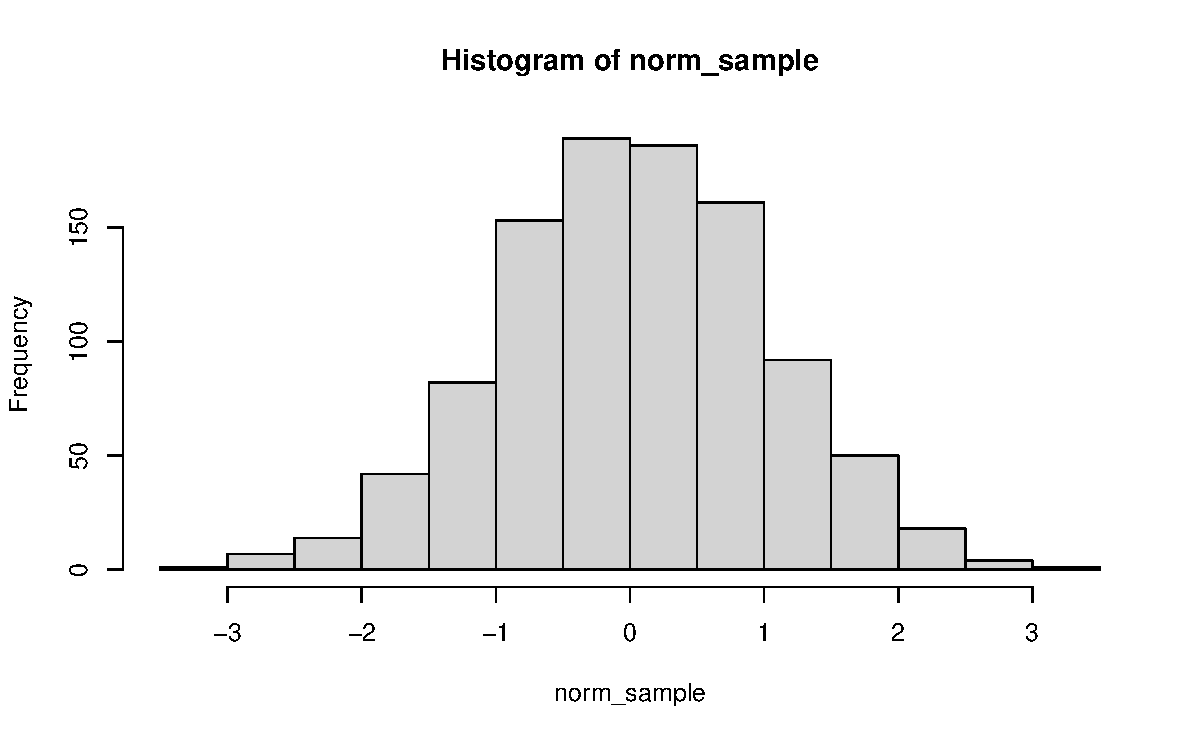
\includegraphics[width=0.7\linewidth]{Data-Analysis-Coursebook_files/figure-latex/unnamed-chunk-41-1} 

}

\caption{Histogram of standard normal distribution}\label{fig:unnamed-chunk-41}
\end{figure}

Now we had to assign the \texttt{norm\_sample} object to use only for a single graph. If you are working on a project it will be confusing to have tons of one time used objects in your \texttt{environment} (Like \texttt{DataFrameAfterCleaningStep1}, \texttt{DataFrameAfterCleaningStep2}, \texttt{DataFrameAfterCleaningStep3}, etc.).

With the pipe operator we can embed several steps into one single workflow. This way we do not have to assign the \texttt{norm\_sample} object. We simple generate the random values AND THEN draw their distribution.

\begin{Shaded}
\begin{Highlighting}[]
\FunctionTok{rnorm}\NormalTok{(}\AttributeTok{n =} \DecValTok{1000}\NormalTok{, }\AttributeTok{mean =} \DecValTok{0}\NormalTok{, }\AttributeTok{sd =} \DecValTok{1}\NormalTok{) }\SpecialCharTok{\%\textgreater{}\%} 
  \FunctionTok{hist}\NormalTok{()}
\end{Highlighting}
\end{Shaded}

\begin{figure}

{\centering 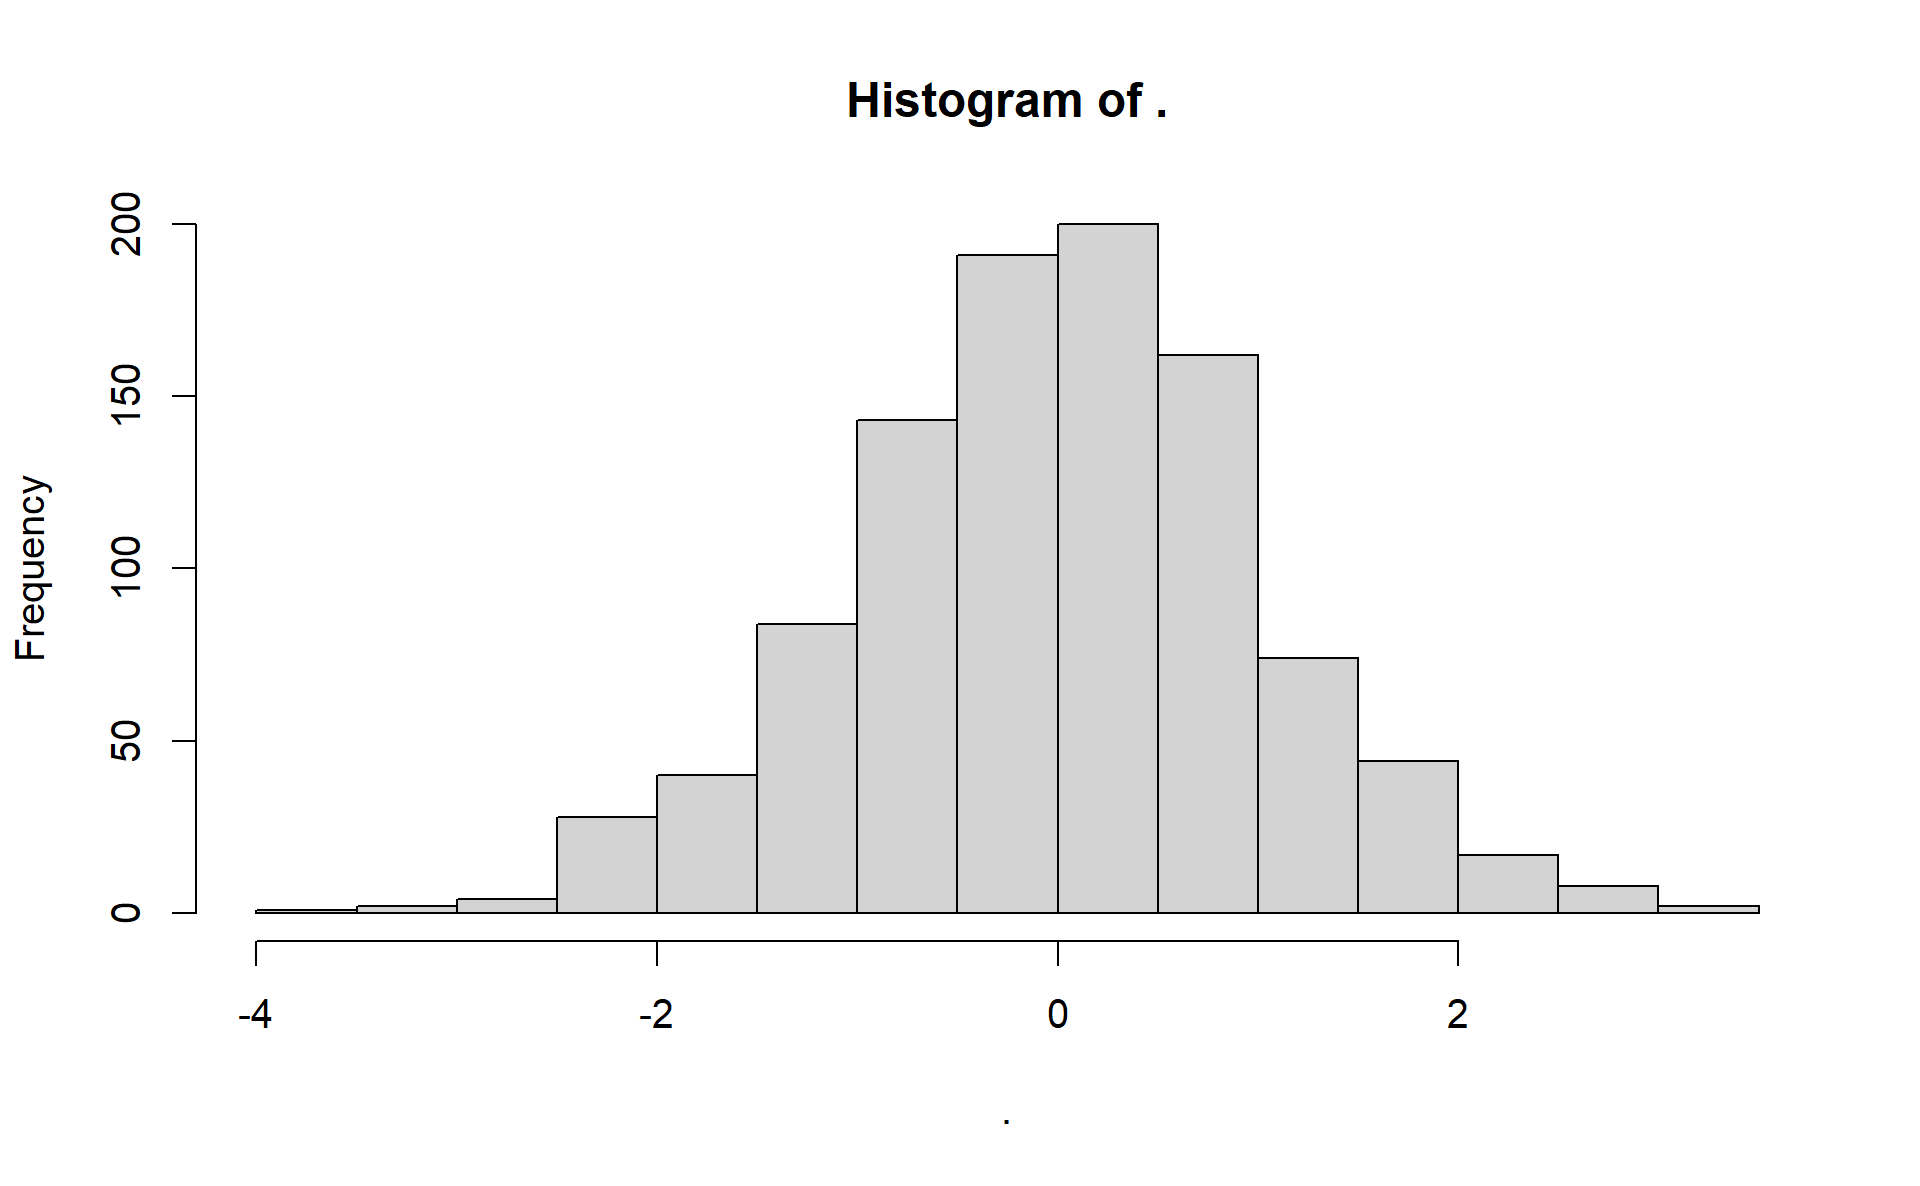
\includegraphics[width=0.7\linewidth]{Data-Analysis-Coursebook_files/figure-latex/unnamed-chunk-42-1} 

}

\caption{Histogram of standard normal distribution using the pipe}\label{fig:unnamed-chunk-42}
\end{figure}

You may see that the title of plot has changed (probably the graph also changed a bit, since chances are low that we generate exactly the 1000 random values). This is because pipe and many other tidyverse function works with a \emph{lambda like} function framework. This means that you can refer to the input value (only if you have only one single input) with \texttt{.}.

Example:

\begin{Shaded}
\begin{Highlighting}[]
\NormalTok{(}\DecValTok{2} \SpecialCharTok{+} \DecValTok{2}\NormalTok{) }\SpecialCharTok{\%\textgreater{}\%} 
\NormalTok{  \{. }\SpecialCharTok{*}\NormalTok{ .\}}
\CommentTok{\#\textgreater{} [1] 16}
\end{Highlighting}
\end{Shaded}

The result is 16, since 2 + 2 = 4, and 4 * 4 equals 16.

The pipe may seem unrelevant first, but this is one of the most powerful tool in R if you have complex data manipulating steps. We will cover the core functions of \texttt{dplyr} in this chapter, which appear in the following video (37:30 - 38:30), but when you are familier with them, you will see the motivation behind the pipe.

\hypertarget{tibble-count-filter-select-arrange}{%
\subsection{Tibble, count, filter, select, arrange}\label{tibble-count-filter-select-arrange}}

\hypertarget{tibble}{%
\subsubsection{Tibble}\label{tibble}}

Let's import a dataset from the \href{https://data.oecd.org/pop/fertility-rates.htm\#indicator-chart}{OECD webpage}. Download the data in csv format and paste it into your working directory.

\begin{Shaded}
\begin{Highlighting}[]
\NormalTok{fertility\_df }\OtherTok{\textless{}{-}} \FunctionTok{read\_csv}\NormalTok{(}\StringTok{"DP\_LIVE\_22092021161631568.csv"}\NormalTok{)}
\end{Highlighting}
\end{Shaded}

\texttt{read\_csv} is importad from the \texttt{readr} package, thus shares its output is adequat to the tidyverse principles. \texttt{fertility\_df} is a data.frame, but it is a \texttt{tibble}, which means that it will be printed nicely on the console: only the first 10 rows appears, and only the amount of columns that can be printed without a linebreak (similar to pandas dataframe in python).

\begin{Shaded}
\begin{Highlighting}[]
\NormalTok{fertility\_df}
\CommentTok{\#\textgreater{} \# A tibble: 3,193 x 8}
\CommentTok{\#\textgreater{}    LOCATION INDICATOR SUBJECT MEASURE   FREQUENCY  TIME Value \textasciigrave{}Flag Codes\textasciigrave{}}
\CommentTok{\#\textgreater{}    \textless{}chr\textgreater{}    \textless{}chr\textgreater{}     \textless{}chr\textgreater{}   \textless{}chr\textgreater{}     \textless{}chr\textgreater{}     \textless{}dbl\textgreater{} \textless{}dbl\textgreater{} \textless{}lgl\textgreater{}       }
\CommentTok{\#\textgreater{}  1 AUS      FERTILITY TOT     CHD\_WOMAN A          1960  3.45 NA          }
\CommentTok{\#\textgreater{}  2 AUS      FERTILITY TOT     CHD\_WOMAN A          1961  3.55 NA          }
\CommentTok{\#\textgreater{}  3 AUS      FERTILITY TOT     CHD\_WOMAN A          1962  3.43 NA          }
\CommentTok{\#\textgreater{}  4 AUS      FERTILITY TOT     CHD\_WOMAN A          1963  3.34 NA          }
\CommentTok{\#\textgreater{}  5 AUS      FERTILITY TOT     CHD\_WOMAN A          1964  3.15 NA          }
\CommentTok{\#\textgreater{}  6 AUS      FERTILITY TOT     CHD\_WOMAN A          1965  2.97 NA          }
\CommentTok{\#\textgreater{}  7 AUS      FERTILITY TOT     CHD\_WOMAN A          1966  2.89 NA          }
\CommentTok{\#\textgreater{}  8 AUS      FERTILITY TOT     CHD\_WOMAN A          1967  2.85 NA          }
\CommentTok{\#\textgreater{}  9 AUS      FERTILITY TOT     CHD\_WOMAN A          1968  2.89 NA          }
\CommentTok{\#\textgreater{} 10 AUS      FERTILITY TOT     CHD\_WOMAN A          1969  2.89 NA          }
\CommentTok{\#\textgreater{} \# ... with 3,183 more rows}
\end{Highlighting}
\end{Shaded}

\hypertarget{count}{%
\subsubsection{Count}\label{count}}

With the \texttt{count} function you can simple \emph{count} the number of appearancesof the levels of a given column. Example:

\begin{Shaded}
\begin{Highlighting}[]
\FunctionTok{count}\NormalTok{(fertility\_df, LOCATION)}
\CommentTok{\#\textgreater{} \# A tibble: 54 x 2}
\CommentTok{\#\textgreater{}    LOCATION     n}
\CommentTok{\#\textgreater{}    \textless{}chr\textgreater{}    \textless{}int\textgreater{}}
\CommentTok{\#\textgreater{}  1 ARG         60}
\CommentTok{\#\textgreater{}  2 AUS         60}
\CommentTok{\#\textgreater{}  3 AUT         61}
\CommentTok{\#\textgreater{}  4 BEL         60}
\CommentTok{\#\textgreater{}  5 BGR         60}
\CommentTok{\#\textgreater{}  6 BRA         60}
\CommentTok{\#\textgreater{}  7 CAN         60}
\CommentTok{\#\textgreater{}  8 CHE         61}
\CommentTok{\#\textgreater{}  9 CHL         60}
\CommentTok{\#\textgreater{} 10 CHN         60}
\CommentTok{\#\textgreater{} \# ... with 44 more rows}
\end{Highlighting}
\end{Shaded}

Now we can see that we have 60 observation from ARG. If you are interested in for which country we have the most datapoints, you can use the \texttt{sort\ =\ TRUE} option.

\begin{Shaded}
\begin{Highlighting}[]
\FunctionTok{count}\NormalTok{(fertility\_df, LOCATION, }\AttributeTok{sort =} \ConstantTok{TRUE}\NormalTok{)}
\CommentTok{\#\textgreater{} \# A tibble: 54 x 2}
\CommentTok{\#\textgreater{}    LOCATION     n}
\CommentTok{\#\textgreater{}    \textless{}chr\textgreater{}    \textless{}int\textgreater{}}
\CommentTok{\#\textgreater{}  1 AUT         61}
\CommentTok{\#\textgreater{}  2 CHE         61}
\CommentTok{\#\textgreater{}  3 CZE         61}
\CommentTok{\#\textgreater{}  4 DNK         61}
\CommentTok{\#\textgreater{}  5 EST         61}
\CommentTok{\#\textgreater{}  6 FIN         61}
\CommentTok{\#\textgreater{}  7 FRA         61}
\CommentTok{\#\textgreater{}  8 LUX         61}
\CommentTok{\#\textgreater{}  9 NOR         61}
\CommentTok{\#\textgreater{} 10 NZL         61}
\CommentTok{\#\textgreater{} \# ... with 44 more rows}
\end{Highlighting}
\end{Shaded}

You can also use the pipe here{[}\^{}It would not be a good solution to assign a new dataframe to each count table{]}

\begin{Shaded}
\begin{Highlighting}[]
\NormalTok{fertility\_df }\SpecialCharTok{\%\textgreater{}\%} \CommentTok{\# \%\textgreater{}\% = the 1st argument of count function is the fertility\_df data.frame}
  \FunctionTok{count}\NormalTok{(LOCATION)}
\CommentTok{\#\textgreater{} \# A tibble: 54 x 2}
\CommentTok{\#\textgreater{}    LOCATION     n}
\CommentTok{\#\textgreater{}    \textless{}chr\textgreater{}    \textless{}int\textgreater{}}
\CommentTok{\#\textgreater{}  1 ARG         60}
\CommentTok{\#\textgreater{}  2 AUS         60}
\CommentTok{\#\textgreater{}  3 AUT         61}
\CommentTok{\#\textgreater{}  4 BEL         60}
\CommentTok{\#\textgreater{}  5 BGR         60}
\CommentTok{\#\textgreater{}  6 BRA         60}
\CommentTok{\#\textgreater{}  7 CAN         60}
\CommentTok{\#\textgreater{}  8 CHE         61}
\CommentTok{\#\textgreater{}  9 CHL         60}
\CommentTok{\#\textgreater{} 10 CHN         60}
\CommentTok{\#\textgreater{} \# ... with 44 more rows}
\end{Highlighting}
\end{Shaded}

You may specifiy multiple columns, this way the frequency of all value combinaton appears.

\begin{Shaded}
\begin{Highlighting}[]
\NormalTok{fertility\_df }\SpecialCharTok{\%\textgreater{}\%} 
  \FunctionTok{count}\NormalTok{(LOCATION, TIME, }\AttributeTok{sort =}\NormalTok{ T)}
\CommentTok{\#\textgreater{} \# A tibble: 3,193 x 3}
\CommentTok{\#\textgreater{}    LOCATION  TIME     n}
\CommentTok{\#\textgreater{}    \textless{}chr\textgreater{}    \textless{}dbl\textgreater{} \textless{}int\textgreater{}}
\CommentTok{\#\textgreater{}  1 ARG       1960     1}
\CommentTok{\#\textgreater{}  2 ARG       1961     1}
\CommentTok{\#\textgreater{}  3 ARG       1962     1}
\CommentTok{\#\textgreater{}  4 ARG       1963     1}
\CommentTok{\#\textgreater{}  5 ARG       1964     1}
\CommentTok{\#\textgreater{}  6 ARG       1965     1}
\CommentTok{\#\textgreater{}  7 ARG       1966     1}
\CommentTok{\#\textgreater{}  8 ARG       1967     1}
\CommentTok{\#\textgreater{}  9 ARG       1968     1}
\CommentTok{\#\textgreater{} 10 ARG       1969     1}
\CommentTok{\#\textgreater{} \# ... with 3,183 more rows}
\end{Highlighting}
\end{Shaded}

Now we see that we have only one observation for each country at a time, so this data frame was originally tidy (this is usually not the case). Let's see for example the Q GDP data from the \href{https://data.oecd.org/gdp/quarterly-gdp.htm}{OECD webpage}.

\begin{Shaded}
\begin{Highlighting}[]
\NormalTok{gdp\_df }\OtherTok{\textless{}{-}} \FunctionTok{read\_csv}\NormalTok{(}\StringTok{"DP\_LIVE\_22092021163414835.csv"}\NormalTok{)}
\end{Highlighting}
\end{Shaded}

Using the \texttt{count} function, we may find that \texttt{MEASURE}, \texttt{SUBJECT} \& \texttt{FREQUENCY} columns have multiple levels.

\begin{Shaded}
\begin{Highlighting}[]
\NormalTok{gdp\_df }\SpecialCharTok{\%\textgreater{}\%} 
  \FunctionTok{count}\NormalTok{(MEASURE, SUBJECT, FREQUENCY)}
\CommentTok{\#\textgreater{} \# A tibble: 5 x 4}
\CommentTok{\#\textgreater{}   MEASURE  SUBJECT FREQUENCY     n}
\CommentTok{\#\textgreater{}   \textless{}chr\textgreater{}    \textless{}chr\textgreater{}   \textless{}chr\textgreater{}     \textless{}int\textgreater{}}
\CommentTok{\#\textgreater{} 1 IDX      VOLIDX  A          1764}
\CommentTok{\#\textgreater{} 2 IDX      VOLIDX  Q          7127}
\CommentTok{\#\textgreater{} 3 PC\_CHGPP TOT     A          2329}
\CommentTok{\#\textgreater{} 4 PC\_CHGPP TOT     Q          9472}
\CommentTok{\#\textgreater{} 5 PC\_CHGPY TOT     Q          9385}
\end{Highlighting}
\end{Shaded}

Let's say we are interested only in the observations where the \texttt{SUBJECT} is equal to TOT (total), \texttt{MEASURE} is equal to PC\_CHGPY (percentage change to previous value) and the \texttt{FREQUENCY} is not equal to A (only quarterly observations). \emph{You can select rows by using the} \texttt{filter} function. Its 1st argument is the dataframe you want to modify, and the other arguments are conditional statements. If all the statements are TRUE, then the row will be selected.

\begin{Shaded}
\begin{Highlighting}[]
\FunctionTok{filter}\NormalTok{(gdp\_df, SUBJECT }\SpecialCharTok{==} \StringTok{"TOT"}\NormalTok{, MEASURE }\SpecialCharTok{==} \StringTok{"PC\_CHGPY"}\NormalTok{, FREQUENCY }\SpecialCharTok{!=} \StringTok{"A"}\NormalTok{)}
\CommentTok{\#\textgreater{} \# A tibble: 9,385 x 8}
\CommentTok{\#\textgreater{}    LOCATION INDICATOR SUBJECT MEASURE  FREQUENCY TIME     Value \textasciigrave{}Flag Codes\textasciigrave{}}
\CommentTok{\#\textgreater{}    \textless{}chr\textgreater{}    \textless{}chr\textgreater{}     \textless{}chr\textgreater{}   \textless{}chr\textgreater{}    \textless{}chr\textgreater{}     \textless{}chr\textgreater{}    \textless{}dbl\textgreater{} \textless{}chr\textgreater{}       }
\CommentTok{\#\textgreater{}  1 DEU      QGDP      TOT     PC\_CHGPY Q         1961{-}Q1  7.45  E           }
\CommentTok{\#\textgreater{}  2 DEU      QGDP      TOT     PC\_CHGPY Q         1961{-}Q2  5.00  E           }
\CommentTok{\#\textgreater{}  3 DEU      QGDP      TOT     PC\_CHGPY Q         1961{-}Q3  3.58  E           }
\CommentTok{\#\textgreater{}  4 DEU      QGDP      TOT     PC\_CHGPY Q         1961{-}Q4  3.00  E           }
\CommentTok{\#\textgreater{}  5 DEU      QGDP      TOT     PC\_CHGPY Q         1962{-}Q1  3.47  E           }
\CommentTok{\#\textgreater{}  6 DEU      QGDP      TOT     PC\_CHGPY Q         1962{-}Q2  5.11  E           }
\CommentTok{\#\textgreater{}  7 DEU      QGDP      TOT     PC\_CHGPY Q         1962{-}Q3  5.47  E           }
\CommentTok{\#\textgreater{}  8 DEU      QGDP      TOT     PC\_CHGPY Q         1962{-}Q4  4.76  E           }
\CommentTok{\#\textgreater{}  9 DEU      QGDP      TOT     PC\_CHGPY Q         1963{-}Q1 {-}0.372 E           }
\CommentTok{\#\textgreater{} 10 DEU      QGDP      TOT     PC\_CHGPY Q         1963{-}Q2  3.02  E           }
\CommentTok{\#\textgreater{} \# ... with 9,375 more rows}
\end{Highlighting}
\end{Shaded}

Just like the \texttt{count}, we use this function with \texttt{\%\textgreater{}\%} operator, and use \texttt{\&} instead of \texttt{,}, but if you wish to use \emph{``OR''}, then you can use \texttt{\textbar{}} between two statement.

\begin{Shaded}
\begin{Highlighting}[]
\NormalTok{gdp\_df }\SpecialCharTok{\%\textgreater{}\%} 
  \FunctionTok{filter}\NormalTok{(SUBJECT }\SpecialCharTok{==} \StringTok{"TOT"} \SpecialCharTok{\&}\NormalTok{ MEASURE }\SpecialCharTok{==} \StringTok{"PC\_CHGPY"} \SpecialCharTok{\&}\NormalTok{ FREQUENCY }\SpecialCharTok{!=} \StringTok{"A"}\NormalTok{)}
\CommentTok{\#\textgreater{} \# A tibble: 9,385 x 8}
\CommentTok{\#\textgreater{}    LOCATION INDICATOR SUBJECT MEASURE  FREQUENCY TIME     Value \textasciigrave{}Flag Codes\textasciigrave{}}
\CommentTok{\#\textgreater{}    \textless{}chr\textgreater{}    \textless{}chr\textgreater{}     \textless{}chr\textgreater{}   \textless{}chr\textgreater{}    \textless{}chr\textgreater{}     \textless{}chr\textgreater{}    \textless{}dbl\textgreater{} \textless{}chr\textgreater{}       }
\CommentTok{\#\textgreater{}  1 DEU      QGDP      TOT     PC\_CHGPY Q         1961{-}Q1  7.45  E           }
\CommentTok{\#\textgreater{}  2 DEU      QGDP      TOT     PC\_CHGPY Q         1961{-}Q2  5.00  E           }
\CommentTok{\#\textgreater{}  3 DEU      QGDP      TOT     PC\_CHGPY Q         1961{-}Q3  3.58  E           }
\CommentTok{\#\textgreater{}  4 DEU      QGDP      TOT     PC\_CHGPY Q         1961{-}Q4  3.00  E           }
\CommentTok{\#\textgreater{}  5 DEU      QGDP      TOT     PC\_CHGPY Q         1962{-}Q1  3.47  E           }
\CommentTok{\#\textgreater{}  6 DEU      QGDP      TOT     PC\_CHGPY Q         1962{-}Q2  5.11  E           }
\CommentTok{\#\textgreater{}  7 DEU      QGDP      TOT     PC\_CHGPY Q         1962{-}Q3  5.47  E           }
\CommentTok{\#\textgreater{}  8 DEU      QGDP      TOT     PC\_CHGPY Q         1962{-}Q4  4.76  E           }
\CommentTok{\#\textgreater{}  9 DEU      QGDP      TOT     PC\_CHGPY Q         1963{-}Q1 {-}0.372 E           }
\CommentTok{\#\textgreater{} 10 DEU      QGDP      TOT     PC\_CHGPY Q         1963{-}Q2  3.02  E           }
\CommentTok{\#\textgreater{} \# ... with 9,375 more rows}
\end{Highlighting}
\end{Shaded}

\hypertarget{mutate}{%
\subsubsection{Mutate}\label{mutate}}

In the \texttt{gdp\_df} dataframe you can find the \texttt{TIME} column and that its class character. Lets say we want to change this to date. Functions related to date are in the \texttt{lubridate} package. Since the values of the \texttt{TIME} column consist of a \emph{y}ear and a \emph{q}uarter, we will use the \texttt{yq} function to change it into date. But we should not forget that this will work only with the datapoints where the \texttt{FREQUENCY} is not annual. So let's keep the previous filter. If we want to modify a given column of a dataframe we should use the \texttt{mutate} function. With the pipe operator we now combine the \texttt{filter} and the \texttt{mutate} command.

\begin{Shaded}
\begin{Highlighting}[]
\NormalTok{gdp\_df }\SpecialCharTok{\%\textgreater{}\%} 
  \FunctionTok{filter}\NormalTok{(SUBJECT }\SpecialCharTok{==} \StringTok{"TOT"} \SpecialCharTok{\&}\NormalTok{ MEASURE }\SpecialCharTok{==} \StringTok{"PC\_CHGPY"} \SpecialCharTok{\&}\NormalTok{ FREQUENCY }\SpecialCharTok{!=} \StringTok{"A"}\NormalTok{) }\SpecialCharTok{\%\textgreater{}\%} 
  \FunctionTok{mutate}\NormalTok{(}\AttributeTok{TIME =}\NormalTok{ lubridate}\SpecialCharTok{::}\FunctionTok{yq}\NormalTok{(TIME))}
\CommentTok{\#\textgreater{} \# A tibble: 9,385 x 8}
\CommentTok{\#\textgreater{}    LOCATION INDICATOR SUBJECT MEASURE  FREQUENCY TIME        Value \textasciigrave{}Flag Codes\textasciigrave{}}
\CommentTok{\#\textgreater{}    \textless{}chr\textgreater{}    \textless{}chr\textgreater{}     \textless{}chr\textgreater{}   \textless{}chr\textgreater{}    \textless{}chr\textgreater{}     \textless{}date\textgreater{}      \textless{}dbl\textgreater{} \textless{}chr\textgreater{}       }
\CommentTok{\#\textgreater{}  1 DEU      QGDP      TOT     PC\_CHGPY Q         1961{-}01{-}01  7.45  E           }
\CommentTok{\#\textgreater{}  2 DEU      QGDP      TOT     PC\_CHGPY Q         1961{-}04{-}01  5.00  E           }
\CommentTok{\#\textgreater{}  3 DEU      QGDP      TOT     PC\_CHGPY Q         1961{-}07{-}01  3.58  E           }
\CommentTok{\#\textgreater{}  4 DEU      QGDP      TOT     PC\_CHGPY Q         1961{-}10{-}01  3.00  E           }
\CommentTok{\#\textgreater{}  5 DEU      QGDP      TOT     PC\_CHGPY Q         1962{-}01{-}01  3.47  E           }
\CommentTok{\#\textgreater{}  6 DEU      QGDP      TOT     PC\_CHGPY Q         1962{-}04{-}01  5.11  E           }
\CommentTok{\#\textgreater{}  7 DEU      QGDP      TOT     PC\_CHGPY Q         1962{-}07{-}01  5.47  E           }
\CommentTok{\#\textgreater{}  8 DEU      QGDP      TOT     PC\_CHGPY Q         1962{-}10{-}01  4.76  E           }
\CommentTok{\#\textgreater{}  9 DEU      QGDP      TOT     PC\_CHGPY Q         1963{-}01{-}01 {-}0.372 E           }
\CommentTok{\#\textgreater{} 10 DEU      QGDP      TOT     PC\_CHGPY Q         1963{-}04{-}01  3.02  E           }
\CommentTok{\#\textgreater{} \# ... with 9,375 more rows}
\end{Highlighting}
\end{Shaded}

Now that \texttt{TIME} is already a date column, we can add an additional condition: we want to analyze only the latest valuse (where the value of \texttt{TIME} is maximum).

\begin{Shaded}
\begin{Highlighting}[]
\NormalTok{gdp\_df }\SpecialCharTok{\%\textgreater{}\%} 
  \FunctionTok{filter}\NormalTok{(SUBJECT }\SpecialCharTok{==} \StringTok{"TOT"} \SpecialCharTok{\&}\NormalTok{ MEASURE }\SpecialCharTok{==} \StringTok{"PC\_CHGPY"} \SpecialCharTok{\&}\NormalTok{ FREQUENCY }\SpecialCharTok{!=} \StringTok{"A"}\NormalTok{) }\SpecialCharTok{\%\textgreater{}\%} 
  \FunctionTok{mutate}\NormalTok{(}\AttributeTok{TIME =}\NormalTok{ lubridate}\SpecialCharTok{::}\FunctionTok{yq}\NormalTok{(TIME)) }\SpecialCharTok{\%\textgreater{}\%} 
  \FunctionTok{filter}\NormalTok{(TIME }\SpecialCharTok{==} \FunctionTok{max}\NormalTok{(TIME)) }
\CommentTok{\#\textgreater{} \# A tibble: 49 x 8}
\CommentTok{\#\textgreater{}    LOCATION INDICATOR SUBJECT MEASURE  FREQUENCY TIME       Value \textasciigrave{}Flag Codes\textasciigrave{}}
\CommentTok{\#\textgreater{}    \textless{}chr\textgreater{}    \textless{}chr\textgreater{}     \textless{}chr\textgreater{}   \textless{}chr\textgreater{}    \textless{}chr\textgreater{}     \textless{}date\textgreater{}     \textless{}dbl\textgreater{} \textless{}chr\textgreater{}       }
\CommentTok{\#\textgreater{}  1 DEU      QGDP      TOT     PC\_CHGPY Q         2021{-}04{-}01  9.41 P           }
\CommentTok{\#\textgreater{}  2 IND      QGDP      TOT     PC\_CHGPY Q         2021{-}04{-}01 20.9  \textless{}NA\textgreater{}        }
\CommentTok{\#\textgreater{}  3 TUR      QGDP      TOT     PC\_CHGPY Q         2021{-}04{-}01 21.4  \textless{}NA\textgreater{}        }
\CommentTok{\#\textgreater{}  4 IDN      QGDP      TOT     PC\_CHGPY Q         2021{-}04{-}01  7.19 \textless{}NA\textgreater{}        }
\CommentTok{\#\textgreater{}  5 LVA      QGDP      TOT     PC\_CHGPY Q         2021{-}04{-}01 10.8  \textless{}NA\textgreater{}        }
\CommentTok{\#\textgreater{}  6 CZE      QGDP      TOT     PC\_CHGPY Q         2021{-}04{-}01  8.18 \textless{}NA\textgreater{}        }
\CommentTok{\#\textgreater{}  7 BRA      QGDP      TOT     PC\_CHGPY Q         2021{-}04{-}01 12.4  \textless{}NA\textgreater{}        }
\CommentTok{\#\textgreater{}  8 POL      QGDP      TOT     PC\_CHGPY Q         2021{-}04{-}01 11.0  \textless{}NA\textgreater{}        }
\CommentTok{\#\textgreater{}  9 MEX      QGDP      TOT     PC\_CHGPY Q         2021{-}04{-}01 19.5  P           }
\CommentTok{\#\textgreater{} 10 CAN      QGDP      TOT     PC\_CHGPY Q         2021{-}04{-}01 12.7  \textless{}NA\textgreater{}        }
\CommentTok{\#\textgreater{} \# ... with 39 more rows}
\end{Highlighting}
\end{Shaded}

Let's where we find the highest values. We have to change the order of the rows with the \texttt{arrange} function. If you want to set decreasing order, then you should put the columns name into the \texttt{desc} command.

\begin{Shaded}
\begin{Highlighting}[]
\NormalTok{gdp\_df }\SpecialCharTok{\%\textgreater{}\%} 
  \FunctionTok{filter}\NormalTok{(SUBJECT }\SpecialCharTok{==} \StringTok{"TOT"} \SpecialCharTok{\&}\NormalTok{ MEASURE }\SpecialCharTok{==} \StringTok{"PC\_CHGPY"} \SpecialCharTok{\&}\NormalTok{ FREQUENCY }\SpecialCharTok{!=} \StringTok{"A"}\NormalTok{) }\SpecialCharTok{\%\textgreater{}\%} 
  \FunctionTok{mutate}\NormalTok{(}\AttributeTok{TIME =}\NormalTok{ lubridate}\SpecialCharTok{::}\FunctionTok{yq}\NormalTok{(TIME)) }\SpecialCharTok{\%\textgreater{}\%} 
  \FunctionTok{filter}\NormalTok{(TIME }\SpecialCharTok{==} \FunctionTok{max}\NormalTok{(TIME)) }\SpecialCharTok{\%\textgreater{}\%}
  \FunctionTok{arrange}\NormalTok{(}\FunctionTok{desc}\NormalTok{(Value)) }
\CommentTok{\#\textgreater{} \# A tibble: 49 x 8}
\CommentTok{\#\textgreater{}    LOCATION INDICATOR SUBJECT MEASURE  FREQUENCY TIME       Value \textasciigrave{}Flag Codes\textasciigrave{}}
\CommentTok{\#\textgreater{}    \textless{}chr\textgreater{}    \textless{}chr\textgreater{}     \textless{}chr\textgreater{}   \textless{}chr\textgreater{}    \textless{}chr\textgreater{}     \textless{}date\textgreater{}     \textless{}dbl\textgreater{} \textless{}chr\textgreater{}       }
\CommentTok{\#\textgreater{}  1 GBR      QGDP      TOT     PC\_CHGPY Q         2021{-}04{-}01  22.2 \textless{}NA\textgreater{}        }
\CommentTok{\#\textgreater{}  2 TUR      QGDP      TOT     PC\_CHGPY Q         2021{-}04{-}01  21.4 \textless{}NA\textgreater{}        }
\CommentTok{\#\textgreater{}  3 IRL      QGDP      TOT     PC\_CHGPY Q         2021{-}04{-}01  21.1 \textless{}NA\textgreater{}        }
\CommentTok{\#\textgreater{}  4 IND      QGDP      TOT     PC\_CHGPY Q         2021{-}04{-}01  20.9 \textless{}NA\textgreater{}        }
\CommentTok{\#\textgreater{}  5 ESP      QGDP      TOT     PC\_CHGPY Q         2021{-}04{-}01  19.8 P           }
\CommentTok{\#\textgreater{}  6 MEX      QGDP      TOT     PC\_CHGPY Q         2021{-}04{-}01  19.5 P           }
\CommentTok{\#\textgreater{}  7 FRA      QGDP      TOT     PC\_CHGPY Q         2021{-}04{-}01  18.7 \textless{}NA\textgreater{}        }
\CommentTok{\#\textgreater{}  8 HUN      QGDP      TOT     PC\_CHGPY Q         2021{-}04{-}01  17.7 \textless{}NA\textgreater{}        }
\CommentTok{\#\textgreater{}  9 NZL      QGDP      TOT     PC\_CHGPY Q         2021{-}04{-}01  17.4 \textless{}NA\textgreater{}        }
\CommentTok{\#\textgreater{} 10 ITA      QGDP      TOT     PC\_CHGPY Q         2021{-}04{-}01  17.3 \textless{}NA\textgreater{}        }
\CommentTok{\#\textgreater{} \# ... with 39 more rows}
\end{Highlighting}
\end{Shaded}

And we want to remove the unused columns. You can select columns with the \texttt{select} function.

\begin{Shaded}
\begin{Highlighting}[]
\NormalTok{gdp\_df }\SpecialCharTok{\%\textgreater{}\%} 
  \FunctionTok{filter}\NormalTok{(SUBJECT }\SpecialCharTok{==} \StringTok{"TOT"} \SpecialCharTok{\&}\NormalTok{ MEASURE }\SpecialCharTok{==} \StringTok{"PC\_CHGPY"} \SpecialCharTok{\&}\NormalTok{ FREQUENCY }\SpecialCharTok{!=} \StringTok{"A"}\NormalTok{) }\SpecialCharTok{\%\textgreater{}\%} 
  \FunctionTok{mutate}\NormalTok{(}\AttributeTok{TIME =}\NormalTok{ lubridate}\SpecialCharTok{::}\FunctionTok{yq}\NormalTok{(TIME)) }\SpecialCharTok{\%\textgreater{}\%} 
  \FunctionTok{filter}\NormalTok{(TIME }\SpecialCharTok{==} \FunctionTok{max}\NormalTok{(TIME)) }\SpecialCharTok{\%\textgreater{}\%} 
  \FunctionTok{arrange}\NormalTok{(}\FunctionTok{desc}\NormalTok{(Value)) }\SpecialCharTok{\%\textgreater{}\%} 
  \FunctionTok{select}\NormalTok{(}\AttributeTok{geo =}\NormalTok{ LOCATION, }\AttributeTok{gdp\_change =}\NormalTok{ Value) }\CommentTok{\# select the LOCATION \& gdp\_change columns}
\CommentTok{\#\textgreater{} \# A tibble: 49 x 2}
\CommentTok{\#\textgreater{}    geo   gdp\_change}
\CommentTok{\#\textgreater{}    \textless{}chr\textgreater{}      \textless{}dbl\textgreater{}}
\CommentTok{\#\textgreater{}  1 GBR         22.2}
\CommentTok{\#\textgreater{}  2 TUR         21.4}
\CommentTok{\#\textgreater{}  3 IRL         21.1}
\CommentTok{\#\textgreater{}  4 IND         20.9}
\CommentTok{\#\textgreater{}  5 ESP         19.8}
\CommentTok{\#\textgreater{}  6 MEX         19.5}
\CommentTok{\#\textgreater{}  7 FRA         18.7}
\CommentTok{\#\textgreater{}  8 HUN         17.7}
\CommentTok{\#\textgreater{}  9 NZL         17.4}
\CommentTok{\#\textgreater{} 10 ITA         17.3}
\CommentTok{\#\textgreater{} \# ... with 39 more rows}
\end{Highlighting}
\end{Shaded}

Alternative notation with select:

\begin{Shaded}
\begin{Highlighting}[]
\NormalTok{gdp\_df }\SpecialCharTok{\%\textgreater{}\%} 
  \FunctionTok{select}\NormalTok{(}\DecValTok{1}\NormalTok{) }\CommentTok{\# select the 1st column}
\CommentTok{\#\textgreater{} \# A tibble: 30,077 x 1}
\CommentTok{\#\textgreater{}    LOCATION}
\CommentTok{\#\textgreater{}    \textless{}chr\textgreater{}   }
\CommentTok{\#\textgreater{}  1 OECD    }
\CommentTok{\#\textgreater{}  2 OECD    }
\CommentTok{\#\textgreater{}  3 OECD    }
\CommentTok{\#\textgreater{}  4 OECD    }
\CommentTok{\#\textgreater{}  5 OECD    }
\CommentTok{\#\textgreater{}  6 OECD    }
\CommentTok{\#\textgreater{}  7 OECD    }
\CommentTok{\#\textgreater{}  8 OECD    }
\CommentTok{\#\textgreater{}  9 OECD    }
\CommentTok{\#\textgreater{} 10 OECD    }
\CommentTok{\#\textgreater{} \# ... with 30,067 more rows}

\NormalTok{gdp\_df }\SpecialCharTok{\%\textgreater{}\%} 
  \FunctionTok{select}\NormalTok{(}\SpecialCharTok{{-}}\DecValTok{1}\NormalTok{) }\CommentTok{\# omit the 1st column}
\CommentTok{\#\textgreater{} \# A tibble: 30,077 x 7}
\CommentTok{\#\textgreater{}    INDICATOR SUBJECT MEASURE  FREQUENCY TIME  Value \textasciigrave{}Flag Codes\textasciigrave{}}
\CommentTok{\#\textgreater{}    \textless{}chr\textgreater{}     \textless{}chr\textgreater{}   \textless{}chr\textgreater{}    \textless{}chr\textgreater{}     \textless{}chr\textgreater{} \textless{}dbl\textgreater{} \textless{}chr\textgreater{}       }
\CommentTok{\#\textgreater{}  1 QGDP      TOT     PC\_CHGPP A         1962   5.70 \textless{}NA\textgreater{}        }
\CommentTok{\#\textgreater{}  2 QGDP      TOT     PC\_CHGPP A         1963   5.20 \textless{}NA\textgreater{}        }
\CommentTok{\#\textgreater{}  3 QGDP      TOT     PC\_CHGPP A         1964   6.38 \textless{}NA\textgreater{}        }
\CommentTok{\#\textgreater{}  4 QGDP      TOT     PC\_CHGPP A         1965   5.35 \textless{}NA\textgreater{}        }
\CommentTok{\#\textgreater{}  5 QGDP      TOT     PC\_CHGPP A         1966   5.75 \textless{}NA\textgreater{}        }
\CommentTok{\#\textgreater{}  6 QGDP      TOT     PC\_CHGPP A         1967   3.96 \textless{}NA\textgreater{}        }
\CommentTok{\#\textgreater{}  7 QGDP      TOT     PC\_CHGPP A         1968   5.92 \textless{}NA\textgreater{}        }
\CommentTok{\#\textgreater{}  8 QGDP      TOT     PC\_CHGPP A         1969   5.57 \textless{}NA\textgreater{}        }
\CommentTok{\#\textgreater{}  9 QGDP      TOT     PC\_CHGPP A         1970   3.94 \textless{}NA\textgreater{}        }
\CommentTok{\#\textgreater{} 10 QGDP      TOT     PC\_CHGPP A         1971   3.70 \textless{}NA\textgreater{}        }
\CommentTok{\#\textgreater{} \# ... with 30,067 more rows}

\NormalTok{gdp\_df }\SpecialCharTok{\%\textgreater{}\%} 
  \FunctionTok{select}\NormalTok{(}\DecValTok{1}\SpecialCharTok{:}\DecValTok{2}\NormalTok{) }\CommentTok{\# select all the columns between the 1st and the 2nd}
\CommentTok{\#\textgreater{} \# A tibble: 30,077 x 2}
\CommentTok{\#\textgreater{}    LOCATION INDICATOR}
\CommentTok{\#\textgreater{}    \textless{}chr\textgreater{}    \textless{}chr\textgreater{}    }
\CommentTok{\#\textgreater{}  1 OECD     QGDP     }
\CommentTok{\#\textgreater{}  2 OECD     QGDP     }
\CommentTok{\#\textgreater{}  3 OECD     QGDP     }
\CommentTok{\#\textgreater{}  4 OECD     QGDP     }
\CommentTok{\#\textgreater{}  5 OECD     QGDP     }
\CommentTok{\#\textgreater{}  6 OECD     QGDP     }
\CommentTok{\#\textgreater{}  7 OECD     QGDP     }
\CommentTok{\#\textgreater{}  8 OECD     QGDP     }
\CommentTok{\#\textgreater{}  9 OECD     QGDP     }
\CommentTok{\#\textgreater{} 10 OECD     QGDP     }
\CommentTok{\#\textgreater{} \# ... with 30,067 more rows}

\NormalTok{gdp\_df }\SpecialCharTok{\%\textgreater{}\%} 
  \FunctionTok{select}\NormalTok{(LOCATION}\SpecialCharTok{:}\NormalTok{TIME) }\CommentTok{\# select all the columns between the LOCATION and the TIME column}
\CommentTok{\#\textgreater{} \# A tibble: 30,077 x 6}
\CommentTok{\#\textgreater{}    LOCATION INDICATOR SUBJECT MEASURE  FREQUENCY TIME }
\CommentTok{\#\textgreater{}    \textless{}chr\textgreater{}    \textless{}chr\textgreater{}     \textless{}chr\textgreater{}   \textless{}chr\textgreater{}    \textless{}chr\textgreater{}     \textless{}chr\textgreater{}}
\CommentTok{\#\textgreater{}  1 OECD     QGDP      TOT     PC\_CHGPP A         1962 }
\CommentTok{\#\textgreater{}  2 OECD     QGDP      TOT     PC\_CHGPP A         1963 }
\CommentTok{\#\textgreater{}  3 OECD     QGDP      TOT     PC\_CHGPP A         1964 }
\CommentTok{\#\textgreater{}  4 OECD     QGDP      TOT     PC\_CHGPP A         1965 }
\CommentTok{\#\textgreater{}  5 OECD     QGDP      TOT     PC\_CHGPP A         1966 }
\CommentTok{\#\textgreater{}  6 OECD     QGDP      TOT     PC\_CHGPP A         1967 }
\CommentTok{\#\textgreater{}  7 OECD     QGDP      TOT     PC\_CHGPP A         1968 }
\CommentTok{\#\textgreater{}  8 OECD     QGDP      TOT     PC\_CHGPP A         1969 }
\CommentTok{\#\textgreater{}  9 OECD     QGDP      TOT     PC\_CHGPP A         1970 }
\CommentTok{\#\textgreater{} 10 OECD     QGDP      TOT     PC\_CHGPP A         1971 }
\CommentTok{\#\textgreater{} \# ... with 30,067 more rows}

\NormalTok{gdp\_df }\SpecialCharTok{\%\textgreater{}\%} 
  \FunctionTok{select}\NormalTok{(TIME, LOCATION, }\FunctionTok{everything}\NormalTok{()) }
\CommentTok{\#\textgreater{} \# A tibble: 30,077 x 8}
\CommentTok{\#\textgreater{}    TIME  LOCATION INDICATOR SUBJECT MEASURE  FREQUENCY Value \textasciigrave{}Flag Codes\textasciigrave{}}
\CommentTok{\#\textgreater{}    \textless{}chr\textgreater{} \textless{}chr\textgreater{}    \textless{}chr\textgreater{}     \textless{}chr\textgreater{}   \textless{}chr\textgreater{}    \textless{}chr\textgreater{}     \textless{}dbl\textgreater{} \textless{}chr\textgreater{}       }
\CommentTok{\#\textgreater{}  1 1962  OECD     QGDP      TOT     PC\_CHGPP A          5.70 \textless{}NA\textgreater{}        }
\CommentTok{\#\textgreater{}  2 1963  OECD     QGDP      TOT     PC\_CHGPP A          5.20 \textless{}NA\textgreater{}        }
\CommentTok{\#\textgreater{}  3 1964  OECD     QGDP      TOT     PC\_CHGPP A          6.38 \textless{}NA\textgreater{}        }
\CommentTok{\#\textgreater{}  4 1965  OECD     QGDP      TOT     PC\_CHGPP A          5.35 \textless{}NA\textgreater{}        }
\CommentTok{\#\textgreater{}  5 1966  OECD     QGDP      TOT     PC\_CHGPP A          5.75 \textless{}NA\textgreater{}        }
\CommentTok{\#\textgreater{}  6 1967  OECD     QGDP      TOT     PC\_CHGPP A          3.96 \textless{}NA\textgreater{}        }
\CommentTok{\#\textgreater{}  7 1968  OECD     QGDP      TOT     PC\_CHGPP A          5.92 \textless{}NA\textgreater{}        }
\CommentTok{\#\textgreater{}  8 1969  OECD     QGDP      TOT     PC\_CHGPP A          5.57 \textless{}NA\textgreater{}        }
\CommentTok{\#\textgreater{}  9 1970  OECD     QGDP      TOT     PC\_CHGPP A          3.94 \textless{}NA\textgreater{}        }
\CommentTok{\#\textgreater{} 10 1971  OECD     QGDP      TOT     PC\_CHGPP A          3.70 \textless{}NA\textgreater{}        }
\CommentTok{\#\textgreater{} \# ... with 30,067 more rows}
  \CommentTok{\# select all the columns, but TIME \& LOCATION to the first place}
\end{Highlighting}
\end{Shaded}

\hypertarget{group_by-summary}{%
\subsection{\texorpdfstring{\texttt{Group\_by}, \texttt{Summary}}{Group\_by, Summary}}\label{group_by-summary}}

Let's see another source for data. You can easily access Eurostat tables with the \texttt{eurostat} package.

\begin{Shaded}
\begin{Highlighting}[]
\NormalTok{eurostat}\SpecialCharTok{::}\FunctionTok{search\_eurostat}\NormalTok{(}\StringTok{"birth"}\NormalTok{)}
\CommentTok{\#\textgreater{} \# A tibble: 275 x 8}
\CommentTok{\#\textgreater{}    title   code  type  \textasciigrave{}last update of\textasciitilde{} \textasciigrave{}last table str\textasciitilde{} \textasciigrave{}data start\textasciigrave{} \textasciigrave{}data end\textasciigrave{}}
\CommentTok{\#\textgreater{}    \textless{}chr\textgreater{}   \textless{}chr\textgreater{} \textless{}chr\textgreater{} \textless{}chr\textgreater{}            \textless{}chr\textgreater{}            \textless{}chr\textgreater{}        \textless{}chr\textgreater{}     }
\CommentTok{\#\textgreater{}  1 Live b\textasciitilde{} demo\textasciitilde{} data\textasciitilde{} 30.06.2021       23.02.2021       1990         2019      }
\CommentTok{\#\textgreater{}  2 Live b\textasciitilde{} demo\textasciitilde{} data\textasciitilde{} 01.07.2021       01.07.2021       2013         2019      }
\CommentTok{\#\textgreater{}  3 Live b\textasciitilde{} demo\textasciitilde{} data\textasciitilde{} 30.06.2021       23.02.2021       1990         2019      }
\CommentTok{\#\textgreater{}  4 Popula\textasciitilde{} cens\textasciitilde{} data\textasciitilde{} 26.08.2015       08.02.2021       2011         2011      }
\CommentTok{\#\textgreater{}  5 Popula\textasciitilde{} cens\textasciitilde{} data\textasciitilde{} 26.08.2015       08.02.2021       2011         2011      }
\CommentTok{\#\textgreater{}  6 Popula\textasciitilde{} cens\textasciitilde{} data\textasciitilde{} 26.08.2015       08.02.2021       2011         2011      }
\CommentTok{\#\textgreater{}  7 Popula\textasciitilde{} cens\textasciitilde{} data\textasciitilde{} 26.08.2015       08.02.2021       2011         2011      }
\CommentTok{\#\textgreater{}  8 Popula\textasciitilde{} cens\textasciitilde{} data\textasciitilde{} 26.08.2015       08.02.2021       2011         2011      }
\CommentTok{\#\textgreater{}  9 Popula\textasciitilde{} lfst\textasciitilde{} data\textasciitilde{} 10.09.2021       27.04.2021       1999         2020      }
\CommentTok{\#\textgreater{} 10 Activi\textasciitilde{} lfst\textasciitilde{} data\textasciitilde{} 10.09.2021       27.04.2021       1999         2020      }
\CommentTok{\#\textgreater{} \# ... with 265 more rows, and 1 more variable: values \textless{}chr\textgreater{}}
\end{Highlighting}
\end{Shaded}

Let's choose the ``Live births by mother's age and NUTS 2 region'' dataset.

\begin{Shaded}
\begin{Highlighting}[]
\NormalTok{livebirth\_eu\_df }\OtherTok{\textless{}{-}}\NormalTok{ eurostat}\SpecialCharTok{::}\FunctionTok{get\_eurostat}\NormalTok{(}\StringTok{"demo\_r\_fagec"}\NormalTok{)}

\NormalTok{livebirth\_eu\_df}
\CommentTok{\#\textgreater{} \# A tibble: 456,956 x 5}
\CommentTok{\#\textgreater{}    unit  age   geo   time       values}
\CommentTok{\#\textgreater{}    \textless{}chr\textgreater{} \textless{}chr\textgreater{} \textless{}chr\textgreater{} \textless{}date\textgreater{}      \textless{}dbl\textgreater{}}
\CommentTok{\#\textgreater{}  1 NR    TOTAL AL    2019{-}01{-}01  28561}
\CommentTok{\#\textgreater{}  2 NR    TOTAL AL0   2019{-}01{-}01  28438}
\CommentTok{\#\textgreater{}  3 NR    TOTAL AL01  2019{-}01{-}01   8909}
\CommentTok{\#\textgreater{}  4 NR    TOTAL AL02  2019{-}01{-}01  12089}
\CommentTok{\#\textgreater{}  5 NR    TOTAL AL03  2019{-}01{-}01   7440}
\CommentTok{\#\textgreater{}  6 NR    TOTAL ALX   2019{-}01{-}01    123}
\CommentTok{\#\textgreater{}  7 NR    TOTAL ALXX  2019{-}01{-}01    123}
\CommentTok{\#\textgreater{}  8 NR    TOTAL AT    2019{-}01{-}01  84952}
\CommentTok{\#\textgreater{}  9 NR    TOTAL AT1   2019{-}01{-}01  36819}
\CommentTok{\#\textgreater{} 10 NR    TOTAL AT11  2019{-}01{-}01   2232}
\CommentTok{\#\textgreater{} \# ... with 456,946 more rows}
\end{Highlighting}
\end{Shaded}

First of all, we are interested in NUTS 2 reginal data. But in this dataset national aggregated values are also published (where the geo codes length is only 2 characters). Let's remove these.

\begin{Shaded}
\begin{Highlighting}[]
\NormalTok{livebirth\_eu\_df }\SpecialCharTok{\%\textgreater{}\%} 
  \FunctionTok{filter}\NormalTok{(}\FunctionTok{str\_length}\NormalTok{(geo) }\SpecialCharTok{!=} \DecValTok{2}\NormalTok{)}
\CommentTok{\#\textgreater{} \# A tibble: 416,961 x 5}
\CommentTok{\#\textgreater{}    unit  age   geo   time       values}
\CommentTok{\#\textgreater{}    \textless{}chr\textgreater{} \textless{}chr\textgreater{} \textless{}chr\textgreater{} \textless{}date\textgreater{}      \textless{}dbl\textgreater{}}
\CommentTok{\#\textgreater{}  1 NR    TOTAL AL0   2019{-}01{-}01  28438}
\CommentTok{\#\textgreater{}  2 NR    TOTAL AL01  2019{-}01{-}01   8909}
\CommentTok{\#\textgreater{}  3 NR    TOTAL AL02  2019{-}01{-}01  12089}
\CommentTok{\#\textgreater{}  4 NR    TOTAL AL03  2019{-}01{-}01   7440}
\CommentTok{\#\textgreater{}  5 NR    TOTAL ALX   2019{-}01{-}01    123}
\CommentTok{\#\textgreater{}  6 NR    TOTAL ALXX  2019{-}01{-}01    123}
\CommentTok{\#\textgreater{}  7 NR    TOTAL AT1   2019{-}01{-}01  36819}
\CommentTok{\#\textgreater{}  8 NR    TOTAL AT11  2019{-}01{-}01   2232}
\CommentTok{\#\textgreater{}  9 NR    TOTAL AT12  2019{-}01{-}01  14652}
\CommentTok{\#\textgreater{} 10 NR    TOTAL AT13  2019{-}01{-}01  19935}
\CommentTok{\#\textgreater{} \# ... with 416,951 more rows}
\end{Highlighting}
\end{Shaded}

We also should remove the aggregated values and keep only the latest one.

\begin{Shaded}
\begin{Highlighting}[]
\NormalTok{livebirth\_eu\_df }\SpecialCharTok{\%\textgreater{}\%} 
  \FunctionTok{filter}\NormalTok{(}\FunctionTok{str\_length}\NormalTok{(geo) }\SpecialCharTok{!=} \DecValTok{2}\NormalTok{) }\SpecialCharTok{\%\textgreater{}\%} 
  \FunctionTok{filter}\NormalTok{(age }\SpecialCharTok{!=} \StringTok{"TOTAL"} \SpecialCharTok{\&}\NormalTok{ time }\SpecialCharTok{==} \StringTok{"2019{-}01{-}01"}\NormalTok{) }\SpecialCharTok{\%\textgreater{}\%} 
  \FunctionTok{filter}\NormalTok{(}\SpecialCharTok{!}\NormalTok{(age }\SpecialCharTok{\%in\%} \FunctionTok{c}\NormalTok{(}\StringTok{"UNK"}\NormalTok{, }\StringTok{"Y\_GE45"}\NormalTok{, }\StringTok{"Y\_GE48"}\NormalTok{, }\StringTok{"Y\_GE50"}\NormalTok{, }\StringTok{"Y\_LT16"}\NormalTok{)))}
\CommentTok{\#\textgreater{} \# A tibble: 14,309 x 5}
\CommentTok{\#\textgreater{}    unit  age    geo   time       values}
\CommentTok{\#\textgreater{}    \textless{}chr\textgreater{} \textless{}chr\textgreater{}  \textless{}chr\textgreater{} \textless{}date\textgreater{}      \textless{}dbl\textgreater{}}
\CommentTok{\#\textgreater{}  1 NR    Y10{-}14 AL0   2019{-}01{-}01     24}
\CommentTok{\#\textgreater{}  2 NR    Y10{-}14 AL01  2019{-}01{-}01      4}
\CommentTok{\#\textgreater{}  3 NR    Y10{-}14 AL02  2019{-}01{-}01     13}
\CommentTok{\#\textgreater{}  4 NR    Y10{-}14 AL03  2019{-}01{-}01      7}
\CommentTok{\#\textgreater{}  5 NR    Y10{-}14 ALX   2019{-}01{-}01      0}
\CommentTok{\#\textgreater{}  6 NR    Y10{-}14 ALXX  2019{-}01{-}01      0}
\CommentTok{\#\textgreater{}  7 NR    Y10{-}14 AT1   2019{-}01{-}01      1}
\CommentTok{\#\textgreater{}  8 NR    Y10{-}14 AT11  2019{-}01{-}01      0}
\CommentTok{\#\textgreater{}  9 NR    Y10{-}14 AT12  2019{-}01{-}01      0}
\CommentTok{\#\textgreater{} 10 NR    Y10{-}14 AT13  2019{-}01{-}01      1}
\CommentTok{\#\textgreater{} \# ... with 14,299 more rows}
\end{Highlighting}
\end{Shaded}

Now our dataset is clean: we have one observation to each geo and age category. Let's suppose we are interested in the total number of birth by the mothers age in EU (I know we would found a table for this). For this we want to sum the values in the \texttt{values} column by age category.

\begin{Shaded}
\begin{Highlighting}[]
\NormalTok{livebirth\_eu\_df }\SpecialCharTok{\%\textgreater{}\%} 
  \FunctionTok{filter}\NormalTok{(}\FunctionTok{str\_length}\NormalTok{(geo) }\SpecialCharTok{!=} \DecValTok{2}\NormalTok{) }\SpecialCharTok{\%\textgreater{}\%} 
  \FunctionTok{filter}\NormalTok{(age }\SpecialCharTok{!=} \StringTok{"TOTAL"} \SpecialCharTok{\&}\NormalTok{ time }\SpecialCharTok{==} \StringTok{"2019{-}01{-}01"}\NormalTok{) }\SpecialCharTok{\%\textgreater{}\%} 
  \FunctionTok{filter}\NormalTok{(}\SpecialCharTok{!}\NormalTok{(age }\SpecialCharTok{\%in\%} \FunctionTok{c}\NormalTok{(}\StringTok{"UNK"}\NormalTok{, }\StringTok{"Y\_GE45"}\NormalTok{, }\StringTok{"Y\_GE48"}\NormalTok{, }\StringTok{"Y\_GE50"}\NormalTok{, }\StringTok{"Y\_LT16"}\NormalTok{))) }\SpecialCharTok{\%\textgreater{}\%} 
  \FunctionTok{group\_by}\NormalTok{(age) }\SpecialCharTok{\%\textgreater{}\%}
  \FunctionTok{summarise}\NormalTok{(}\AttributeTok{values =} \FunctionTok{sum}\NormalTok{(values))}
\end{Highlighting}
\end{Shaded}

\begin{tabular}{l|r}
\hline
age & values\\
\hline
Y10-14 & 5337\\
\hline
Y15 & 13440\\
\hline
Y16 & 30049\\
\hline
Y17 & 60282\\
\hline
Y18 & 106563\\
\hline
Y19 & 172655\\
\hline
Y20 & 244849\\
\hline
Y21 & 308539\\
\hline
Y22 & 378984\\
\hline
Y23 & 450972\\
\hline
Y24 & 542341\\
\hline
Y25 & 649112\\
\hline
Y26 & 757241\\
\hline
Y27 & 867143\\
\hline
Y28 & 971229\\
\hline
Y29 & 1053152\\
\hline
Y30 & 1089894\\
\hline
Y31 & 1099205\\
\hline
Y32 & 1044856\\
\hline
Y33 & 979962\\
\hline
Y34 & 903304\\
\hline
Y35 & 811897\\
\hline
Y36 & 707466\\
\hline
Y37 & 597897\\
\hline
Y38 & 489777\\
\hline
Y39 & 385349\\
\hline
Y40 & 281512\\
\hline
Y41 & 192645\\
\hline
Y42 & 124356\\
\hline
Y43 & 73296\\
\hline
Y44 & 43848\\
\hline
Y45 & 23717\\
\hline
Y46 & 12628\\
\hline
Y47 & 7172\\
\hline
Y48 & 4354\\
\hline
Y49 & 2922\\
\hline
\end{tabular}

\hypertarget{pivot-longerwider}{%
\subsection{Pivot longer/wider}\label{pivot-longerwider}}

Let's assume we are interested in the growth rate of fertility in each country. First, we should write a function to calculate growth rates (chain index).

\begin{Shaded}
\begin{Highlighting}[]
\NormalTok{chain\_index }\OtherTok{\textless{}{-}} \ControlFlowTok{function}\NormalTok{(x) \{}
\NormalTok{  scales}\SpecialCharTok{::}\FunctionTok{percent}\NormalTok{(x}\SpecialCharTok{/}\FunctionTok{lag}\NormalTok{(x)}\SpecialCharTok{{-}}\DecValTok{1}\NormalTok{, }\AttributeTok{accuracy =}\NormalTok{ .}\DecValTok{01}\NormalTok{)}
  \CommentTok{\# lag: previous observation}
\NormalTok{\}}
\end{Highlighting}
\end{Shaded}

Example:

\begin{Shaded}
\begin{Highlighting}[]
\NormalTok{x }\OtherTok{\textless{}{-}} \FunctionTok{c}\NormalTok{(}\DecValTok{100}\NormalTok{, }\DecValTok{107}\NormalTok{, }\DecValTok{105}\NormalTok{, }\DecValTok{110}\NormalTok{)}

\FunctionTok{chain\_index}\NormalTok{(x)}
\CommentTok{\#\textgreater{} [1] NA       "7.00\%"  "{-}1.87\%" "4.76\%"}
\end{Highlighting}
\end{Shaded}

\begin{Shaded}
\begin{Highlighting}[]
\NormalTok{fertility\_df }\SpecialCharTok{\%\textgreater{}\%} 
  \FunctionTok{select}\NormalTok{(LOCATION, TIME, Value) }\SpecialCharTok{\%\textgreater{}\%} 
  \FunctionTok{mutate}\NormalTok{(}\AttributeTok{GrowthRate =} \FunctionTok{chain\_index}\NormalTok{(Value))}
\end{Highlighting}
\end{Shaded}

(I hided the rest of the table)

\begin{tabular}{l|r|r|l}
\hline
LOCATION & TIME & Value & GrowthRate\\
\hline
AUS & 1960 & 3.45 & NA\\
\hline
AUS & 1961 & 3.55 & 2.90\%\\
\hline
AUS & 1962 & 3.43 & -3.38\%\\
\hline
AUS & 1963 & 3.34 & -2.62\%\\
\hline
AUS & 1964 & 3.15 & -5.69\%\\
\hline
AUS & 1965 & 2.97 & -5.71\%\\
\hline
AUS & 1966 & 2.89 & -2.69\%\\
\hline
AUS & 1967 & 2.85 & -1.38\%\\
\hline
AUS & 1968 & 2.89 & 1.40\%\\
\hline
AUS & 1969 & 2.89 & 0.00\%\\
\hline
AUS & 1970 & 2.86 & -1.04\%\\
\hline
AUS & 1971 & 2.95 & 3.15\%\\
\hline
AUS & 1972 & 2.74 & -7.12\%\\
\hline
AUS & 1973 & 2.49 & -9.12\%\\
\hline
AUS & 1974 & 2.32 & -6.83\%\\
\hline
AUS & 1975 & 2.15 & -7.33\%\\
\hline
AUS & 1976 & 2.06 & -4.19\%\\
\hline
AUS & 1977 & 2.01 & -2.43\%\\
\hline
AUS & 1978 & 1.95 & -2.99\%\\
\hline
AUS & 1979 & 1.91 & -2.05\%\\
\hline
AUS & 1980 & 1.89 & -1.05\%\\
\hline
AUS & 1981 & 1.94 & 2.65\%\\
\hline
AUS & 1982 & 1.93 & -0.52\%\\
\hline
AUS & 1983 & 1.92 & -0.52\%\\
\hline
AUS & 1984 & 1.84 & -4.17\%\\
\hline
AUS & 1985 & 1.92 & 4.35\%\\
\hline
AUS & 1986 & 1.87 & -2.60\%\\
\hline
AUS & 1987 & 1.85 & -1.07\%\\
\hline
AUS & 1988 & 1.83 & -1.08\%\\
\hline
AUS & 1989 & 1.84 & 0.55\%\\
\hline
AUS & 1990 & 1.90 & 3.26\%\\
\hline
AUS & 1991 & 1.85 & -2.63\%\\
\hline
AUS & 1992 & 1.89 & 2.16\%\\
\hline
AUS & 1993 & 1.86 & -1.59\%\\
\hline
AUS & 1994 & 1.84 & -1.08\%\\
\hline
AUS & 1995 & 1.82 & -1.09\%\\
\hline
AUS & 1996 & 1.80 & -1.10\%\\
\hline
AUS & 1997 & 1.78 & -1.11\%\\
\hline
AUS & 1998 & 1.76 & -1.12\%\\
\hline
AUS & 1999 & 1.76 & 0.00\%\\
\hline
AUS & 2000 & 1.76 & 0.00\%\\
\hline
AUS & 2001 & 1.73 & -1.70\%\\
\hline
AUS & 2002 & 1.77 & 2.31\%\\
\hline
AUS & 2003 & 1.77 & 0.00\%\\
\hline
AUS & 2004 & 1.78 & 0.56\%\\
\hline
AUS & 2005 & 1.85 & 3.93\%\\
\hline
AUS & 2006 & 1.88 & 1.62\%\\
\hline
AUS & 2007 & 1.99 & 5.85\%\\
\hline
AUS & 2008 & 2.02 & 1.51\%\\
\hline
AUS & 2009 & 1.97 & -2.48\%\\
\hline
AUS & 2010 & 1.95 & -1.02\%\\
\hline
AUS & 2011 & 1.92 & -1.54\%\\
\hline
AUS & 2012 & 1.93 & 0.52\%\\
\hline
AUS & 2013 & 1.88 & -2.59\%\\
\hline
AUS & 2014 & 1.79 & -4.79\%\\
\hline
AUS & 2015 & 1.79 & 0.00\%\\
\hline
AUS & 2016 & 1.79 & 0.00\%\\
\hline
AUS & 2017 & 1.74 & -2.79\%\\
\hline
AUS & 2018 & 1.74 & 0.00\%\\
\hline
AUS & 2019 & 1.66 & -4.60\%\\
\hline
AUT & 1960 & 2.69 & 62.05\%\\
\hline
AUT & 1961 & 2.78 & 3.35\%\\
\hline
AUT & 1962 & 2.80 & 0.72\%\\
\hline
AUT & 1963 & 2.82 & 0.71\%\\
\hline
AUT & 1964 & 2.79 & -1.06\%\\
\hline
AUT & 1965 & 2.70 & -3.23\%\\
\hline
AUT & 1966 & 2.66 & -1.48\%\\
\hline
AUT & 1967 & 2.62 & -1.50\%\\
\hline
AUT & 1968 & 2.58 & -1.53\%\\
\hline
AUT & 1969 & 2.49 & -3.49\%\\
\hline
\end{tabular}

But the problem comes at the \texttt{GrowthRate} at AUT in 1960, since now (check in the table):

\[\text{Growth}_{\text{AUT}, 1960} = \frac{\text{AUS}_{2019}}{\text{AUT}_{1960}}\]

We can easily solve this by transforming the structure of the table. We need to make the table \textbf{wider} in this case, with the \texttt{pivot\_wider}. this function will create a new column to each level of a seleceted variable.

\begin{Shaded}
\begin{Highlighting}[]
\NormalTok{fertility\_df }\SpecialCharTok{\%\textgreater{}\%} 
  \FunctionTok{select}\NormalTok{(}\AttributeTok{geo =}\NormalTok{ LOCATION, }\AttributeTok{time =}\NormalTok{ TIME, }\AttributeTok{fertility =}\NormalTok{ Value) }\SpecialCharTok{\%\textgreater{}\%} 
  \FunctionTok{pivot\_wider}\NormalTok{(}\AttributeTok{names\_from =} \StringTok{"geo"}\NormalTok{, }\AttributeTok{values\_from =} \StringTok{"fertility"}\NormalTok{)}
\CommentTok{\#\textgreater{} \# A tibble: 61 x 55}
\CommentTok{\#\textgreater{}     time   AUS   AUT   BEL   CAN   CZE   DNK   FIN   FRA   DEU   GRC   HUN   ISL}
\CommentTok{\#\textgreater{}    \textless{}dbl\textgreater{} \textless{}dbl\textgreater{} \textless{}dbl\textgreater{} \textless{}dbl\textgreater{} \textless{}dbl\textgreater{} \textless{}dbl\textgreater{} \textless{}dbl\textgreater{} \textless{}dbl\textgreater{} \textless{}dbl\textgreater{} \textless{}dbl\textgreater{} \textless{}dbl\textgreater{} \textless{}dbl\textgreater{} \textless{}dbl\textgreater{}}
\CommentTok{\#\textgreater{}  1  1960  3.45  2.69  2.54  3.9   2.11  2.54  2.71  2.74  2.37  2.23  2.02  4.26}
\CommentTok{\#\textgreater{}  2  1961  3.55  2.78  2.63  3.84  2.13  2.55  2.65  2.82  2.44  2.13  1.94  3.88}
\CommentTok{\#\textgreater{}  3  1962  3.43  2.8   2.59  3.76  2.14  2.54  2.66  2.8   2.44  2.16  1.79  3.98}
\CommentTok{\#\textgreater{}  4  1963  3.34  2.82  2.68  3.67  2.33  2.64  2.66  2.9   2.51  2.14  1.82  3.98}
\CommentTok{\#\textgreater{}  5  1964  3.15  2.79  2.72  3.5   2.36  2.6   2.58  2.91  2.53  2.24  1.8   3.86}
\CommentTok{\#\textgreater{}  6  1965  2.97  2.7   2.62  3.15  2.18  2.61  2.46  2.85  2.5   2.25  1.81  3.71}
\CommentTok{\#\textgreater{}  7  1966  2.89  2.66  2.52  2.81  2.01  2.62  2.4   2.8   2.51  2.32  1.88  3.58}
\CommentTok{\#\textgreater{}  8  1967  2.85  2.62  2.41  2.6   1.9   2.35  2.32  2.67  2.45  2.45  2.01  3.28}
\CommentTok{\#\textgreater{}  9  1968  2.89  2.58  2.31  2.45  1.83  2.12  2.15  2.59  2.36  2.42  2.06  3.07}
\CommentTok{\#\textgreater{} 10  1969  2.89  2.49  2.28  2.4   1.86  2     1.94  2.53  2.21  2.36  2.04  2.99}
\CommentTok{\#\textgreater{} \# ... with 51 more rows, and 42 more variables: IRL \textless{}dbl\textgreater{}, ITA \textless{}dbl\textgreater{},}
\CommentTok{\#\textgreater{} \#   JPN \textless{}dbl\textgreater{}, KOR \textless{}dbl\textgreater{}, LUX \textless{}dbl\textgreater{}, MEX \textless{}dbl\textgreater{}, NLD \textless{}dbl\textgreater{}, NZL \textless{}dbl\textgreater{},}
\CommentTok{\#\textgreater{} \#   NOR \textless{}dbl\textgreater{}, POL \textless{}dbl\textgreater{}, PRT \textless{}dbl\textgreater{}, SVK \textless{}dbl\textgreater{}, ESP \textless{}dbl\textgreater{}, SWE \textless{}dbl\textgreater{},}
\CommentTok{\#\textgreater{} \#   CHE \textless{}dbl\textgreater{}, TUR \textless{}dbl\textgreater{}, GBR \textless{}dbl\textgreater{}, USA \textless{}dbl\textgreater{}, BRA \textless{}dbl\textgreater{}, CHL \textless{}dbl\textgreater{},}
\CommentTok{\#\textgreater{} \#   CHN \textless{}dbl\textgreater{}, EST \textless{}dbl\textgreater{}, IND \textless{}dbl\textgreater{}, IDN \textless{}dbl\textgreater{}, ISR \textless{}dbl\textgreater{}, RUS \textless{}dbl\textgreater{},}
\CommentTok{\#\textgreater{} \#   SVN \textless{}dbl\textgreater{}, ZAF \textless{}dbl\textgreater{}, COL \textless{}dbl\textgreater{}, LVA \textless{}dbl\textgreater{}, LTU \textless{}dbl\textgreater{}, ARG \textless{}dbl\textgreater{},}
\CommentTok{\#\textgreater{} \#   BGR \textless{}dbl\textgreater{}, HRV \textless{}dbl\textgreater{}, CYP \textless{}dbl\textgreater{}, MLT \textless{}dbl\textgreater{}, ROU \textless{}dbl\textgreater{}, SAU \textless{}dbl\textgreater{}, ...}
\end{Highlighting}
\end{Shaded}

If we use the \texttt{chain\_index} function now on all the columns, then we can avoid the previous bug. You can use a function on all columns (except on the first) with the \texttt{mutate\_at} function.

\begin{Shaded}
\begin{Highlighting}[]
\NormalTok{fertility\_df }\SpecialCharTok{\%\textgreater{}\%} 
  \FunctionTok{select}\NormalTok{(}\AttributeTok{geo =}\NormalTok{ LOCATION, }\AttributeTok{time =}\NormalTok{ TIME, }\AttributeTok{fertility =}\NormalTok{ Value) }\SpecialCharTok{\%\textgreater{}\%} 
  \FunctionTok{pivot\_wider}\NormalTok{(}\AttributeTok{names\_from =} \StringTok{"geo"}\NormalTok{, }\AttributeTok{values\_from =} \StringTok{"fertility"}\NormalTok{) }\SpecialCharTok{\%\textgreater{}\%} 
  \FunctionTok{mutate\_at}\NormalTok{(}\SpecialCharTok{{-}}\DecValTok{1}\NormalTok{, chain\_index)}
\CommentTok{\#\textgreater{} \# A tibble: 61 x 55}
\CommentTok{\#\textgreater{}     time AUS   AUT   BEL   CAN   CZE   DNK   FIN   FRA   DEU   GRC   HUN   ISL  }
\CommentTok{\#\textgreater{}    \textless{}dbl\textgreater{} \textless{}chr\textgreater{} \textless{}chr\textgreater{} \textless{}chr\textgreater{} \textless{}chr\textgreater{} \textless{}chr\textgreater{} \textless{}chr\textgreater{} \textless{}chr\textgreater{} \textless{}chr\textgreater{} \textless{}chr\textgreater{} \textless{}chr\textgreater{} \textless{}chr\textgreater{} \textless{}chr\textgreater{}}
\CommentTok{\#\textgreater{}  1  1960 \textless{}NA\textgreater{}  \textless{}NA\textgreater{}  \textless{}NA\textgreater{}  \textless{}NA\textgreater{}  \textless{}NA\textgreater{}  \textless{}NA\textgreater{}  \textless{}NA\textgreater{}  \textless{}NA\textgreater{}  \textless{}NA\textgreater{}  \textless{}NA\textgreater{}  \textless{}NA\textgreater{}  \textless{}NA\textgreater{} }
\CommentTok{\#\textgreater{}  2  1961 2.90\% 3.35\% 3.54\% {-}1.5\textasciitilde{} 0.95\% 0.39\% {-}2.2\textasciitilde{} 2.92\% 2.95\% {-}4.4\textasciitilde{} {-}3.9\textasciitilde{} {-}8.9\textasciitilde{}}
\CommentTok{\#\textgreater{}  3  1962 {-}3.3\textasciitilde{} 0.72\% {-}1.5\textasciitilde{} {-}2.0\textasciitilde{} 0.47\% {-}0.3\textasciitilde{} 0.38\% {-}0.7\textasciitilde{} 0.00\% 1.41\% {-}7.7\textasciitilde{} 2.58\%}
\CommentTok{\#\textgreater{}  4  1963 {-}2.6\textasciitilde{} 0.71\% 3.47\% {-}2.3\textasciitilde{} 8.88\% 3.94\% 0.00\% 3.57\% 2.87\% {-}0.9\textasciitilde{} 1.68\% 0.00\%}
\CommentTok{\#\textgreater{}  5  1964 {-}5.6\textasciitilde{} {-}1.0\textasciitilde{} 1.49\% {-}4.6\textasciitilde{} 1.29\% {-}1.5\textasciitilde{} {-}3.0\textasciitilde{} 0.34\% 0.80\% 4.67\% {-}1.1\textasciitilde{} {-}3.0\textasciitilde{}}
\CommentTok{\#\textgreater{}  6  1965 {-}5.7\textasciitilde{} {-}3.2\textasciitilde{} {-}3.6\textasciitilde{} {-}10.\textasciitilde{} {-}7.6\textasciitilde{} 0.38\% {-}4.6\textasciitilde{} {-}2.0\textasciitilde{} {-}1.1\textasciitilde{} 0.45\% 0.56\% {-}3.8\textasciitilde{}}
\CommentTok{\#\textgreater{}  7  1966 {-}2.6\textasciitilde{} {-}1.4\textasciitilde{} {-}3.8\textasciitilde{} {-}10.\textasciitilde{} {-}7.8\textasciitilde{} 0.38\% {-}2.4\textasciitilde{} {-}1.7\textasciitilde{} 0.40\% 3.11\% 3.87\% {-}3.5\textasciitilde{}}
\CommentTok{\#\textgreater{}  8  1967 {-}1.3\textasciitilde{} {-}1.5\textasciitilde{} {-}4.3\textasciitilde{} {-}7.4\textasciitilde{} {-}5.4\textasciitilde{} {-}10.\textasciitilde{} {-}3.3\textasciitilde{} {-}4.6\textasciitilde{} {-}2.3\textasciitilde{} 5.60\% 6.91\% {-}8.3\textasciitilde{}}
\CommentTok{\#\textgreater{}  9  1968 1.40\% {-}1.5\textasciitilde{} {-}4.1\textasciitilde{} {-}5.7\textasciitilde{} {-}3.6\textasciitilde{} {-}9.7\textasciitilde{} {-}7.3\textasciitilde{} {-}3.0\textasciitilde{} {-}3.6\textasciitilde{} {-}1.2\textasciitilde{} 2.49\% {-}6.4\textasciitilde{}}
\CommentTok{\#\textgreater{} 10  1969 0.00\% {-}3.4\textasciitilde{} {-}1.3\textasciitilde{} {-}2.0\textasciitilde{} 1.64\% {-}5.6\textasciitilde{} {-}9.7\textasciitilde{} {-}2.3\textasciitilde{} {-}6.3\textasciitilde{} {-}2.4\textasciitilde{} {-}0.9\textasciitilde{} {-}2.6\textasciitilde{}}
\CommentTok{\#\textgreater{} \# ... with 51 more rows, and 42 more variables: IRL \textless{}chr\textgreater{}, ITA \textless{}chr\textgreater{},}
\CommentTok{\#\textgreater{} \#   JPN \textless{}chr\textgreater{}, KOR \textless{}chr\textgreater{}, LUX \textless{}chr\textgreater{}, MEX \textless{}chr\textgreater{}, NLD \textless{}chr\textgreater{}, NZL \textless{}chr\textgreater{},}
\CommentTok{\#\textgreater{} \#   NOR \textless{}chr\textgreater{}, POL \textless{}chr\textgreater{}, PRT \textless{}chr\textgreater{}, SVK \textless{}chr\textgreater{}, ESP \textless{}chr\textgreater{}, SWE \textless{}chr\textgreater{},}
\CommentTok{\#\textgreater{} \#   CHE \textless{}chr\textgreater{}, TUR \textless{}chr\textgreater{}, GBR \textless{}chr\textgreater{}, USA \textless{}chr\textgreater{}, BRA \textless{}chr\textgreater{}, CHL \textless{}chr\textgreater{},}
\CommentTok{\#\textgreater{} \#   CHN \textless{}chr\textgreater{}, EST \textless{}chr\textgreater{}, IND \textless{}chr\textgreater{}, IDN \textless{}chr\textgreater{}, ISR \textless{}chr\textgreater{}, RUS \textless{}chr\textgreater{},}
\CommentTok{\#\textgreater{} \#   SVN \textless{}chr\textgreater{}, ZAF \textless{}chr\textgreater{}, COL \textless{}chr\textgreater{}, LVA \textless{}chr\textgreater{}, LTU \textless{}chr\textgreater{}, ARG \textless{}chr\textgreater{},}
\CommentTok{\#\textgreater{} \#   BGR \textless{}chr\textgreater{}, HRV \textless{}chr\textgreater{}, CYP \textless{}chr\textgreater{}, MLT \textless{}chr\textgreater{}, ROU \textless{}chr\textgreater{}, SAU \textless{}chr\textgreater{}, ...}
\end{Highlighting}
\end{Shaded}

And now let's transform the table to its original structure. You can do this with the \texttt{pivot\_longer} column.

\begin{Shaded}
\begin{Highlighting}[]
\NormalTok{fertility\_df }\SpecialCharTok{\%\textgreater{}\%} 
  \FunctionTok{select}\NormalTok{(}\AttributeTok{geo =}\NormalTok{ LOCATION, }\AttributeTok{time =}\NormalTok{ TIME, }\AttributeTok{fertility =}\NormalTok{ Value) }\SpecialCharTok{\%\textgreater{}\%} 
  \FunctionTok{pivot\_wider}\NormalTok{(}\AttributeTok{names\_from =} \StringTok{"geo"}\NormalTok{, }\AttributeTok{values\_from =} \StringTok{"fertility"}\NormalTok{) }\SpecialCharTok{\%\textgreater{}\%} 
  \FunctionTok{mutate\_at}\NormalTok{(}\SpecialCharTok{{-}}\DecValTok{1}\NormalTok{, chain\_index) }\SpecialCharTok{\%\textgreater{}\%} 
  \FunctionTok{pivot\_longer}\NormalTok{(}\SpecialCharTok{{-}}\DecValTok{1}\NormalTok{, }\AttributeTok{names\_to =} \StringTok{"geo"}\NormalTok{, }\AttributeTok{values\_to =} \StringTok{"fertility"}\NormalTok{)}
\CommentTok{\#\textgreater{} \# A tibble: 3,294 x 3}
\CommentTok{\#\textgreater{}     time geo   fertility}
\CommentTok{\#\textgreater{}    \textless{}dbl\textgreater{} \textless{}chr\textgreater{} \textless{}chr\textgreater{}    }
\CommentTok{\#\textgreater{}  1  1960 AUS   \textless{}NA\textgreater{}     }
\CommentTok{\#\textgreater{}  2  1960 AUT   \textless{}NA\textgreater{}     }
\CommentTok{\#\textgreater{}  3  1960 BEL   \textless{}NA\textgreater{}     }
\CommentTok{\#\textgreater{}  4  1960 CAN   \textless{}NA\textgreater{}     }
\CommentTok{\#\textgreater{}  5  1960 CZE   \textless{}NA\textgreater{}     }
\CommentTok{\#\textgreater{}  6  1960 DNK   \textless{}NA\textgreater{}     }
\CommentTok{\#\textgreater{}  7  1960 FIN   \textless{}NA\textgreater{}     }
\CommentTok{\#\textgreater{}  8  1960 FRA   \textless{}NA\textgreater{}     }
\CommentTok{\#\textgreater{}  9  1960 DEU   \textless{}NA\textgreater{}     }
\CommentTok{\#\textgreater{} 10  1960 GRC   \textless{}NA\textgreater{}     }
\CommentTok{\#\textgreater{} \# ... with 3,284 more rows}
\end{Highlighting}
\end{Shaded}

\hypertarget{group_modify}{%
\subsection{\texorpdfstring{\texttt{Group\_modify}}{Group\_modify}}\label{group_modify}}

Alternativly, we could solve this problem if we split the data frame into 63 individual data frames (one for each country). If you use the following syntax, you will get the correct results:

\begin{Shaded}
\begin{Highlighting}[]
\NormalTok{fertility\_df }\SpecialCharTok{\%\textgreater{}\%} 
  \FunctionTok{select}\NormalTok{(}\AttributeTok{geo =}\NormalTok{ LOCATION, }\AttributeTok{time =}\NormalTok{ TIME, }\AttributeTok{fertility =}\NormalTok{ Value) }\SpecialCharTok{\%\textgreater{}\%} 
  \FunctionTok{arrange}\NormalTok{(time) }\SpecialCharTok{\%\textgreater{}\%} 
  \FunctionTok{group\_by}\NormalTok{(geo) }\SpecialCharTok{\%\textgreater{}\%} 
  \FunctionTok{group\_modify}\NormalTok{(}\SpecialCharTok{\textasciitilde{}} \FunctionTok{mutate}\NormalTok{(.x, }\AttributeTok{fertility\_growth =} \FunctionTok{chain\_index}\NormalTok{(fertility)), }\AttributeTok{.keep =}\NormalTok{ F)}
\end{Highlighting}
\end{Shaded}

\begin{tabular}{l|r|r|l}
\hline
geo & time & fertility & fertility\_growth\\
\hline
ARG & 1960 & 3.11 & NA\\
\hline
ARG & 1961 & 3.10 & -0.32\%\\
\hline
ARG & 1962 & 3.09 & -0.32\%\\
\hline
ARG & 1963 & 3.08 & -0.32\%\\
\hline
ARG & 1964 & 3.07 & -0.32\%\\
\hline
ARG & 1965 & 3.06 & -0.33\%\\
\hline
ARG & 1966 & 3.05 & -0.33\%\\
\hline
ARG & 1967 & 3.05 & 0.00\%\\
\hline
ARG & 1968 & 3.05 & 0.00\%\\
\hline
ARG & 1969 & 3.06 & 0.33\%\\
\hline
ARG & 1970 & 3.08 & 0.65\%\\
\hline
ARG & 1971 & 3.11 & 0.97\%\\
\hline
ARG & 1972 & 3.15 & 1.29\%\\
\hline
ARG & 1973 & 3.20 & 1.59\%\\
\hline
ARG & 1974 & 3.25 & 1.56\%\\
\hline
ARG & 1975 & 3.30 & 1.54\%\\
\hline
ARG & 1976 & 3.34 & 1.21\%\\
\hline
ARG & 1977 & 3.36 & 0.60\%\\
\hline
ARG & 1978 & 3.36 & 0.00\%\\
\hline
ARG & 1979 & 3.34 & -0.60\%\\
\hline
ARG & 1980 & 3.30 & -1.20\%\\
\hline
ARG & 1981 & 3.25 & -1.52\%\\
\hline
ARG & 1982 & 3.20 & -1.54\%\\
\hline
ARG & 1983 & 3.16 & -1.25\%\\
\hline
ARG & 1984 & 3.12 & -1.27\%\\
\hline
ARG & 1985 & 3.10 & -0.64\%\\
\hline
ARG & 1986 & 3.08 & -0.65\%\\
\hline
ARG & 1987 & 3.06 & -0.65\%\\
\hline
ARG & 1988 & 3.04 & -0.65\%\\
\hline
ARG & 1989 & 3.02 & -0.66\%\\
\hline
ARG & 1990 & 3.00 & -0.66\%\\
\hline
ARG & 1991 & 2.97 & -1.00\%\\
\hline
ARG & 1992 & 2.93 & -1.35\%\\
\hline
ARG & 1993 & 2.88 & -1.71\%\\
\hline
ARG & 1994 & 2.83 & -1.74\%\\
\hline
ARG & 1995 & 2.77 & -2.12\%\\
\hline
ARG & 1996 & 2.72 & -1.81\%\\
\hline
ARG & 1997 & 2.67 & -1.84\%\\
\hline
ARG & 1998 & 2.62 & -1.87\%\\
\hline
ARG & 1999 & 2.58 & -1.53\%\\
\hline
ARG & 2000 & 2.54 & -1.55\%\\
\hline
ARG & 2001 & 2.51 & -1.18\%\\
\hline
ARG & 2002 & 2.49 & -0.80\%\\
\hline
ARG & 2003 & 2.46 & -1.20\%\\
\hline
ARG & 2004 & 2.44 & -0.81\%\\
\hline
ARG & 2005 & 2.42 & -0.82\%\\
\hline
ARG & 2006 & 2.40 & -0.83\%\\
\hline
ARG & 2007 & 2.38 & -0.83\%\\
\hline
ARG & 2008 & 2.37 & -0.42\%\\
\hline
ARG & 2009 & 2.36 & -0.42\%\\
\hline
ARG & 2010 & 2.35 & -0.42\%\\
\hline
ARG & 2011 & 2.34 & -0.43\%\\
\hline
ARG & 2012 & 2.33 & -0.43\%\\
\hline
ARG & 2013 & 2.32 & -0.43\%\\
\hline
ARG & 2014 & 2.31 & -0.43\%\\
\hline
ARG & 2015 & 2.30 & -0.43\%\\
\hline
ARG & 2016 & 2.29 & -0.43\%\\
\hline
ARG & 2017 & 2.28 & -0.44\%\\
\hline
ARG & 2018 & 2.26 & -0.88\%\\
\hline
ARG & 2019 & 2.25 & -0.44\%\\
\hline
AUS & 1960 & 3.45 & NA\\
\hline
AUS & 1961 & 3.55 & 2.90\%\\
\hline
AUS & 1962 & 3.43 & -3.38\%\\
\hline
AUS & 1963 & 3.34 & -2.62\%\\
\hline
AUS & 1964 & 3.15 & -5.69\%\\
\hline
AUS & 1965 & 2.97 & -5.71\%\\
\hline
AUS & 1966 & 2.89 & -2.69\%\\
\hline
AUS & 1967 & 2.85 & -1.38\%\\
\hline
AUS & 1968 & 2.89 & 1.40\%\\
\hline
AUS & 1969 & 2.89 & 0.00\%\\
\hline
\end{tabular}

\hypertarget{exercise}{%
\subsection{Exercise}\label{exercise}}

You have to get to know your classmates to solve this exercise.

\begin{enumerate}
\def\labelenumi{\arabic{enumi}.}
\item
  Create a new .Rmd file
\item
  Import the da\_q.csv data into R with relative referencing (see Chapter \ref{data-import})
\item
  Write down the information you know about at least 3 of your teammates (Names are neccesary) as text in the \texttt{.Rmd}.
\item
  Write R codes to find the teammates (write also comments in the code\footnote{``A comment always writes down the why, not the what''}) using only base R function (tools you have learned in the 1st seminar).
\item
  Write R codes to find the teammates using dplyr function (tools you have learned in the 2nd seminar)
\end{enumerate}

\textbf{You found your teammate if the output of an R code is correct ID number of the person.}

Example:

\begin{Shaded}
\begin{Highlighting}[]
\NormalTok{df}
\CommentTok{\#\textgreater{} \# A tibble: 21 x 11}
\CommentTok{\#\textgreater{}       ID \textasciigrave{}What is your zod\textasciitilde{} \textasciigrave{}Do you prefer \textasciitilde{} \textasciigrave{}What experience\textasciitilde{} \textasciigrave{}How many slices\textasciitilde{}}
\CommentTok{\#\textgreater{}    \textless{}dbl\textgreater{} \textless{}chr\textgreater{}              \textless{}chr\textgreater{}            \textless{}chr\textgreater{}             \textless{}chr\textgreater{}            }
\CommentTok{\#\textgreater{}  1     1 leo                dogs             I am familier wi\textasciitilde{} 8                }
\CommentTok{\#\textgreater{}  2     2 taurus             Dogd             I have some expe\textasciitilde{} 12               }
\CommentTok{\#\textgreater{}  3     3 pisces             Both             I do not have an\textasciitilde{} Depends on size.\textasciitilde{}}
\CommentTok{\#\textgreater{}  4     4 taurus             neither          I do not have an\textasciitilde{} 2                }
\CommentTok{\#\textgreater{}  5     5 aquarius           dogs             I have some expe\textasciitilde{} 3                }
\CommentTok{\#\textgreater{}  6     6 leo                Cats             I am familier wi\textasciitilde{} 4                }
\CommentTok{\#\textgreater{}  7     7 virgo              Cats             I am familier wi\textasciitilde{} 4                }
\CommentTok{\#\textgreater{}  8     8 virgo              Dogs             I learnt R in un\textasciitilde{} 4                }
\CommentTok{\#\textgreater{}  9     9 taurus             dogs             I learnt R in un\textasciitilde{} 3                }
\CommentTok{\#\textgreater{} 10    10 cancer             dogs             I do not have an\textasciitilde{} 2                }
\CommentTok{\#\textgreater{} \# ... with 11 more rows, and 6 more variables: Do you wear glasses?2 \textless{}chr\textgreater{},}
\CommentTok{\#\textgreater{} \#   How many countries have you been to so far? \textless{}dbl\textgreater{},}
\CommentTok{\#\textgreater{} \#   How many instagram followers do you have? (zero, if you do not have an account) \textless{}chr\textgreater{},}
\CommentTok{\#\textgreater{} \#   How many brothers and sisters do you have? \textless{}chr\textgreater{},}
\CommentTok{\#\textgreater{} \#   What is your batteries current charge level? (0{-}100) \textless{}chr\textgreater{},}
\CommentTok{\#\textgreater{} \#   What is the traditional food in your country? (you can mention more, if you wish) \textless{}chr\textgreater{}}
\end{Highlighting}
\end{Shaded}

\emph{I am from Hungary, and the national food in Hungary is gulash.}

\begin{Shaded}
\begin{Highlighting}[]
\NormalTok{df }\SpecialCharTok{\%\textgreater{}\%} 
  \FunctionTok{filter}\NormalTok{(}\FunctionTok{str\_detect}\NormalTok{(}\StringTok{\textasciigrave{}}\AttributeTok{What is the traditional food in your country? (you can mention more, if you wish)}\StringTok{\textasciigrave{}}\NormalTok{, }\StringTok{"gulash"}\NormalTok{)) }\SpecialCharTok{\%\textgreater{}\%} 
  \FunctionTok{pull}\NormalTok{(ID)}
\CommentTok{\#\textgreater{} [1] 1}
\end{Highlighting}
\end{Shaded}

\emph{So my ID number is 1.}

Of course, you can not choose me. :)

  \bibliography{references.bib}

\end{document}
